% Created 2024-02-04 Κυρ 17:47
% Intended LaTeX compiler: pdflatex
\documentclass[11pt]{article}
\usepackage[utf8]{inputenc}
\usepackage[T1]{fontenc}
\usepackage{graphicx}
\usepackage{longtable}
\usepackage{wrapfig}
\usepackage{rotating}
\usepackage[normalem]{ulem}
\usepackage{amsmath}
\usepackage{amssymb}
\usepackage{capt-of}
\usepackage{hyperref}
\usepackage{booktabs}
\usepackage{import}
\usepackage[LGR, T1]{fontenc}
\usepackage[greek, english, american]{babel}
\usepackage{alphabeta}
\usepackage{esint}
\usepackage{mathtools}
\usepackage{esdiff}
\usepackage{makeidx}
\usepackage{glossaries}
\usepackage{newfloat}
\usepackage{minted}
\usepackage[a4paper, margin=3cm]{geometry}
\usepackage{chemfig}
\usepackage{svg}
\author{Vidianos Giannitsis}
\date{\today}
\title{Notebook for metabolic pathway prediction}
\hypersetup{
 pdfauthor={Vidianos Giannitsis},
 pdftitle={Notebook for metabolic pathway prediction},
 pdfkeywords={},
 pdfsubject={},
 pdfcreator={Emacs 29.2 (Org mode 9.6.15)}, 
 pdflang={English}}
\makeatletter
\newcommand{\citeprocitem}[2]{\hyper@linkstart{cite}{citeproc_bib_item_#1}#2\hyper@linkend}
\makeatother

\usepackage[notquote]{hanging}
\begin{document}

\maketitle
\tableofcontents


\section{Description of the core concepts}
\label{sec:orga9e9f91}
This notebook is about a personal project of mine, which is mostly done as a learning experience in Julia, but if succesful can have application in my thesis (hence why it is in this directory). The idea is that since we know from literature every pathway a mixed culture fermentation can follow, if we have data for the input and output of either a continuous (in steady state) or batch reactor, we can try to find which pathways were followed and to what extent in each case.

This example can be made into an optimization problem as the extent to which each pathway is followed can be considered the parameters of the simulator and with an L2 loss between experimental data and the output of the simulator, we can optimize it with the classic SciML toolchain.

This can be very useful both for understanding the behaviour of a mixed culture of microorganisms and how they behave in different conditions but also can have very large application in modelling. Modelling mixed cultures is in general fairly hard because of the large amount of processes that can happen, but if we can quantify to what extent each process happens, it makes modelling much easier.

\section{Primitives}
\label{sec:orga422e71}
\subsection{Molar mass definition}
\label{sec:org6476d80}
Since we generally measure concentration in g/l, but reactions are described in molar terms, a very important primitive to implement is molar mass. We define molar mass for a general C\textsubscript{a}H\textsubscript{b}O\textsubscript{c}N\textsubscript{d}S\textsubscript{e} compound with the function

\begin{minted}[breaklines=true,breakanywhere=true]{julia}
# Primitive to calculate molar mass
function molar_mass(; C=0, H=0, O=0, N=0, S=0)
mass = 12C + H + 16O + 14N + 32S
end

\end{minted}

\subsection{Molar mass of substances used}
\label{sec:orgd787e8c}
and then calculate molar mass for all substances used in the system.

\begin{minted}[breaklines=true,breakanywhere=true]{julia}

# Calculate the molar masses of all used substances
function m_glucose()
molar_mass(C=6, H=12, O=6)
end

function m_fructose()
molar_mass(C=6, H=12, O=6)
end

function m_sucrose()
molar_mass(C=12, H=24, O=12)
end

function m_pyruvate()
molar_mass(C=3, H=4, O=3)
end

function m_hydrogen()
molar_mass(H=2)
end

function m_oxygen()
    molar_mass(O=2)
end

function m_co2()
molar_mass(C=1, O=2)
end

function m_water()
molar_mass(H=2, O=1)
end

function m_acetate()
molar_mass(C=2, H=4, O=2)
end

function m_propionate()
molar_mass(C=3, H=6, O=2)
end

function m_butyrate()
molar_mass(C=4, H=8, O=2)
end

function m_ethanol()
molar_mass(C=2, H=6, O=1)
end

function m_lactate()
molar_mass(C=3, H=6, O=3)
end

function m_succinate()
molar_mass(C=4, H=6, O=4)
end

function m_formate()
molar_mass(C=1, H=2, O=2)
end

function m_acetaldehyde()
molar_mass(C=2, H=4, O=1)
end

function m_acetone()
molar_mass(C=3, H=6, O=1)
end

function m_butanol()
molar_mass(C=4, H=10, O=1)
end

function m_valerate()
molar_mass(C=5, H=10, O=2)
end

\end{minted}

\subsection{Concentration to mass}
\label{sec:orgdb6214d}
Since we define molar mass, we can easily convert moles to mass and opposite. However, what we typically measure is concentration, so we also need a function to convert mass to concentration, which is easy as concentration to mass is multiplication with volume and the opposite is division. This is shown below

\begin{minted}[breaklines=true,breakanywhere=true]{julia}

function conc_to_mass(st, volume)
new_st = NamedTuple{keys(st)}(values(st).*volume)
end

function mass_to_conc(st, volume)
new_st = NamedTuple{keys(st)}(values(st)./volume)
end

\end{minted}

\section{Core pathways}
\label{sec:org6a77985}
Then, we can start writing down the metabolic pathways which can happen in this system. The concept is that they all operate in a variable named st (state), which is a named tuple holding the concentration of each compound and return a new state of how the concentrations changed due to this process. Furthermore, they all have one (or multiple) goals, which describe to what extent each reaction is followed.

\subsection{Initial state}
\label{sec:org1fd0c50}
Therefore, we first need an initial state. A test state used for a lot of what is implemented here is displayed below.

\begin{minted}[breaklines=true,breakanywhere=true]{julia}

state = (glucose = 16.0, pyruvate = 0.0, hydrogen = 0.0, water = 700.0, co2 = 0.0,
        acetate = 0.0, propionate = 0.0, butyrate = 0.0, ethanol = 0.0,
        lactate = 0.0, succinate = 0.0, formate = 0.0, acetaldehyde = 0.0,
        fructose = 0.0, sucrose = 0.0, butanol = 0.0, acetone = 0.0,
        valerate = 0.0, oxygen = 0.0)

\end{minted}

\subsection{Glycolysis definition and explanation}
\label{sec:org71f81c7}
After that, we can start writing down reactions. The first reaction we define is glycolysis, the pathway through which glucose is converted to pyruvate, hydrogen and energy. 

\begin{minted}[breaklines=true,breakanywhere=true]{julia}

function glycolysis(st; goal = (; glucose = 0.0))
stoic = (glucose = -1, pyruvate = +2, hydrogen = +2)
mass_stoic = (glucose = stoic.glucose*m_glucose(),
                pyruvate = stoic.pyruvate*m_pyruvate(),
                hydrogen = stoic.hydrogen*m_hydrogen())
goal.glucose <= st.glucose || error("Glucose is not sufficient for this goal")
change = (goal.glucose - st.glucose)/mass_stoic.glucose
new_st = merge(st,
                (glucose = goal.glucose,
                pyruvate = st.pyruvate + change*mass_stoic.pyruvate,
                hydrogen = st.hydrogen + change*mass_stoic.hydrogen))
end

\end{minted}

The logic of the function is we define the stoichiometry, which is known, convert it to mass stoichiometry with the molar mass primitives defined above, find the factor \texttt{change} which calculates the conversion of the reaction in mass terms, from the goal given and update the state so that all compounds are changed by this variable times the mass stoichiometric coefficient. For the variable for which goal is defined, its value can more simply be the value of goal. It also runs an error check if the goal of glucose is larger than the glucose in the initial state. Since it is consumed, it cannot be more than its initial value, so the function should give an error if this is given. The logic of all other core reactions is the same, so it won't be explained again below. 

\subsection{Other sugars}
\label{sec:org61804f5}
However, in a lot of cases we don't have only glucose. The case study I am doing contains sucrose and fructose, but other sugars could be similarly defined. Sucrose is hydrolyzed to an equimolar mixture of glucose and fructose, while fructose enters the EMP pathway (glycolysis) producing glyceraldehyde-3-phosphate, which is an intermediate of pyruvate. Since this system tries to look at a bigger picture and not every intermediate of the process, the implementation of fructolysis will be that fructose isomerises to glucose and goes through glycolysis. Theoretically it is not correct, but with the amount of abstracted detail we have assumed, it does not give any error. Below are there implementations.

\begin{minted}[breaklines=true,breakanywhere=true]{julia}

function sucrose_hydrolysis(st; goal = (; sucrose = 0.0))
stoic = (sucrose = -1, glucose = +1, fructose = +1)
mass_stoic = (sucrose = stoic.sucrose*m_sucrose(),
                glucose = stoic.glucose*m_glucose(),
                fructose = stoic.fructose*m_fructose())
goal.sucrose <= st.sucrose || error("Sucrose is not sufficient for this goal")
change = (goal.sucrose - st.sucrose)/mass_stoic.sucrose
new_st = merge(st,
                (sucrose = goal.sucrose,
                glucose = st.glucose + change*mass_stoic.glucose,
                fructose = st.fructose + change*mass_stoic.fructose))
end

function fructolysis(st; goal = (; fructose = 0.0))
stoic = (fructose = -1, glucose = +1)
mass_stoic = (fructose = stoic.fructose*m_fructose(),
                glucose = stoic.glucose*m_glucose())
goal.fructose <= st.fructose || error("Fructose is not sufficient for this goal")
change = (goal.fructose - st.fructose)/mass_stoic.fructose
fruc_st = merge(st,
                (fructose = goal.fructose,
                glucose = st.glucose + change*mass_stoic.glucose))
new_st = glycolysis(fruc_st, goal = (; glucose = st.glucose))
end

\end{minted}

\section{Pathways of pyruvate consumption}
\label{sec:orgc2b8663}
As mentioned, pyruvate is the core intermediate of the process, produced during glycolysis. There are many pathways it can partake in, producing different products depending on conditions. The core ones (abstracting intermediates of the processes) are:

\begin{itemize}
\item Pyruvate + Water -> Acetate + CO2 + H2
\item Pyruvate -> Acetaldehyde + CO2
\item 2Pyruvate -> Butyrate + 2CO2
\item Pyruvate + H2 -> Lactate
\item Pyruvate + CO2 + H2 -> Succinate
\item 2Pyruvate + 2H\textsubscript{2} -> Water + Butanol + 2CO\textsubscript{2}
\item 2Pyruvate + Water -> 3CO2 + 2H\textsubscript{2} + Acetone
\end{itemize}

\begin{minted}[breaklines=true,breakanywhere=true]{julia}


function pyruv_to_acetate(st; goal = (; pyruvate = 0.0))
stoic = (pyruvate = -1, water = -1, acetate= +1, hydrogen = +1, co2=+1)
mass_stoic = (pyruvate = stoic.pyruvate*m_pyruvate(),
                water = stoic.water*m_water(),
                acetate = stoic.acetate*m_acetate(),
                hydrogen = stoic.hydrogen*m_hydrogen(),
                co2 = stoic.co2*m_co2())
goal.pyruvate <= st.pyruvate || error("Pyruvate is not sufficient for this goal")
change = (goal.pyruvate - st.pyruvate)/mass_stoic.pyruvate
new_st = merge(st,
                (pyruvate = goal.pyruvate,
                water = st.water + change*mass_stoic.water,
                acetate = st.acetate + change*mass_stoic.acetate,
                hydrogen = st.hydrogen + change*mass_stoic.hydrogen,
                co2 = st.co2 + change*mass_stoic.co2))
end

function pyruv_to_acetaldehyde(st; goal = (; pyruvate = 0.0))
stoic = (pyruvate = -1, acetaldehyde = +1, co2 = +1)
mass_stoic = (pyruvate = stoic.pyruvate*m_pyruvate(),
                acetaldehyde = stoic.acetaldehyde*m_acetaldehyde(),
                co2 = stoic.co2*m_co2())
goal.pyruvate <= st.pyruvate || error("Pyruvate is not sufficient for this goal")
change = (goal.pyruvate - st.pyruvate)/mass_stoic.pyruvate
new_st = merge(st,
                (pyruvate = goal.pyruvate,
                acetaldehyde = st.acetaldehyde + change*mass_stoic.acetaldehyde,
                co2 = st.co2 + change*mass_stoic.co2))
end


function pyruv_to_butyr(st; goal = (; pyruvate = 0.0))
stoic = (pyruvate = -2, butyrate = +1, co2 = +2)
mass_stoic = (pyruvate = stoic.pyruvate*m_pyruvate(),
                butyrate = stoic.butyrate*m_butyrate(),
                co2 = stoic.co2*m_co2())
goal.pyruvate <= st.pyruvate || error("Pyruvate is not sufficient for this goal")
change = (goal.pyruvate - st.pyruvate)/mass_stoic.pyruvate
new_st = merge(st,
                (pyruvate = goal.pyruvate,
                butyrate = st.butyrate + change*mass_stoic.butyrate,
                co2 = st.co2 + change*mass_stoic.co2))
end

function pyruv_to_butanol(st; goal = (; pyruvate = 0.0))
stoic = (pyruvate = -2, hydrogen = -2, water = +1, butanol = +1, co2 = +2)
mass_stoic = (pyruvate = stoic.pyruvate*m_pyruvate(),
                hydrogen = stoic.hydrogen*m_hydrogen(),
                water = stoic.water*m_water(),
                butanol = stoic.butanol*m_butanol(),
                co2 = stoic.co2*m_co2())
goal.pyruvate <= st.pyruvate || error("Pyruvate is not sufficient for this goal")
change = (goal.pyruvate - st.pyruvate)/mass_stoic.pyruvate
abs(change*mass_stoic.hydrogen) <= st.hydrogen || error("Hydrogen is not sufficient for this goal")
new_st = merge(st,
                (pyruvate = goal.pyruvate,
                butanol = st.butanol + change*mass_stoic.butanol,
                hydrogen = st.hydrogen + change*mass_stoic.hydrogen,
                co2 = st.co2 + change*mass_stoic.co2,
                water = st.water + change*mass_stoic.water))
end

function pyruv_to_acetone(st; goal = (; pyruvate = 0.0))
stoic = (pyruvate = -2, water = -1, co2 = +3, hydrogen = +2, acetone = +1)
mass_stoic = (pyruvate = stoic.pyruvate*m_pyruvate(),
                water = stoic.water*m_water(),
                hydrogen = stoic.hydrogen*m_hydrogen(),
                co2 = stoic.co2*m_co2(),
                acetone = stoic.acetone*m_acetone())
goal.pyruvate <= st.pyruvate || error("Pyruvate is not sufficient for this goal")
change = (goal.pyruvate - st.pyruvate)/mass_stoic.pyruvate
new_st = merge(st,
                (pyruvate = goal.pyruvate,
                water = st.water + change*mass_stoic.water,
                co2 = st.co2 + change*mass_stoic.co2,
                hydrogen = st.hydrogen + change*mass_stoic.hydrogen,
                acetone = st.acetone + change*mass_stoic.acetone))
end

function pyruv_to_lact(st; goal = (; pyruvate = 0.0))
stoic = (pyruvate = -1, hydrogen = -1, lactate = +1)
mass_stoic = (pyruvate = stoic.pyruvate*m_pyruvate(),
                hydrogen = stoic.hydrogen*m_hydrogen(),
                lactate = stoic.lactate*m_lactate())
goal.pyruvate <= st.pyruvate || error("Pyruvate is not sufficient for this goal")
change = (goal.pyruvate - st.pyruvate)/mass_stoic.pyruvate
abs(change*mass_stoic.hydrogen) <= st.hydrogen || error("Hydrogen is not sufficient for this goal")
new_st = merge(st,
                (pyruvate = goal.pyruvate,
                hydrogen = st.hydrogen + change*mass_stoic.hydrogen,
                lactate = st.lactate + change*mass_stoic.lactate))
end


function pyruv_to_succin(st; goal = (; pyruvate = 0.0))
stoic = (pyruvate = -1, co2 = -1, hydrogen = -2, succinate = +1, water = +1)
mass_stoic = (pyruvate = stoic.pyruvate*m_pyruvate(),
                co2 = stoic.co2*m_co2(),
                hydrogen = stoic.hydrogen*m_hydrogen(),
                succinate = stoic.succinate*m_succinate(),
                water = stoic.water*m_water())
goal.pyruvate <= st.pyruvate || error("Pyruvate is not sufficient for this goal")
change = (goal.pyruvate - st.pyruvate)/mass_stoic.pyruvate
abs(change*mass_stoic.hydrogen) <= st.hydrogen || error("Hydrogen is not sufficient for this goal")
abs(change*mass_stoic.co2) <= st.co2 || error("CO2 is not sufficient for this goal")
new_st = merge(st,
                (pyruvate = goal.pyruvate,
                co2 = st.co2 + change*mass_stoic.co2,
                hydrogen = st.hydrogen + change*mass_stoic.hydrogen,
                succinate = st.succinate + change*mass_stoic.succinate,
                water = st.water + change*mass_stoic.water))
end 

\end{minted}

\section{Other pathways stemming from glycolysis}
\label{sec:orgd205f67}
However, there are also some other important reactions that are in these pathways as the above products are in some cases intermediates for the production of something else. The reactions taking some of these products and converting them to other products are: 

\begin{itemize}
\item Acetaldehyde + H2 -> Ethanol
\item Lactate + H2 -> Propionate
\item Succinate + CO2 -> Propionate
\item Formate <-> CO2 + H2
\item Propionate + 2CO2 + 6H2 -> Valerate
\end{itemize}

and the code for their implementation can be seen below
\begin{minted}[breaklines=true,breakanywhere=true]{julia}


function acetaldehyde_to_ethanol(st; goal = (; acetaldehyde = 0.0))
stoic = (acetaldehyde = -1, hydrogen = -1, ethanol = +1)
mass_stoic = (acetaldehyde = stoic.acetaldehyde*m_acetaldehyde(),
                hydrogen = stoic.hydrogen*m_hydrogen(),
                ethanol = stoic.ethanol*m_ethanol())
goal.acetaldehyde <= st.acetaldehyde || error("Acetaldehyde is not sufficient for this goal")
change = (goal.acetaldehyde - st.acetaldehyde)/mass_stoic.acetaldehyde
abs(change*mass_stoic.hydrogen) <= st.hydrogen || error("Hydrogen is not sufficient for this goal")
new_st = merge(st,
                (acetaldehyde = goal.acetaldehyde,
                hydrogen = st.hydrogen + change*mass_stoic.hydrogen,
                ethanol = st.ethanol + change*mass_stoic.ethanol))
end


function lact_to_propionate(st; goal = (; lactate = 0.0))
stoic = (lactate = -1, hydrogen = -1, propionate = +1)
mass_stoic = (lactate = stoic.lactate*m_lactate(),
                hydrogen = stoic.hydrogen*m_hydrogen(),
                propionate = stoic.propionate*m_propionate())
goal.lactate <= st.lactate || error("Lactate is not sufficient for this goal")
change = (goal.lactate - st.lactate)/mass_stoic.lactate
abs(change*mass_stoic.hydrogen) <= st.hydrogen || error("Hydrogen is not sufficient for this goal")
new_st = merge(st,
                (lactate = goal.lactate,
                hydrogen = st.hydrogen + change*mass_stoic.hydrogen,
                propionate = st.propionate + change*mass_stoic.propionate))
end


function succin_to_propionate(st; goal = (; succinate = 0.0))
stoic = (succinate = -1, propionate = +1, co2 = +1)
mass_stoic = (succinate = stoic.succinate*m_succinate(),
                propionate = stoic.propionate*m_propionate(),
                co2 = stoic.co2*m_co2())
goal.succinate <= st.succinate || error("Succinate is not sufficient for this goal")
change = (goal.succinate - st.succinate)/mass_stoic.succinate
new_st = merge(st,
                (succinate = goal.succinate,
                propionate = st.propionate + change*mass_stoic.propionate,
                co2 = st.co2 + change*mass_stoic.co2))
end

# The formate balance isn't exactly like all the other reactions where
# the goal is the main reactant. It is a reaction very close to
# equilibrium that in pH near neutral or higher is favored on
# formate. If you expect that formate will be produced, you can give a
# goal that formate has this concentration and it will remove enough
# co2 and hydrogen for it to be feasible. Since it is common for none
# to be produced, the default value will be expect that none will be
# produced.
function formate_balance(st; goal = (; formate = 0.0))
stoic = (co2 = -1, hydrogen = -1, formate = +1)
mass_stoic = (co2 = stoic.co2*m_co2(),
                hydrogen = stoic.hydrogen*m_hydrogen(),
                formate = stoic.formate*m_formate())
change = (goal.formate - st.formate)/mass_stoic.formate
abs(change*mass_stoic.hydrogen) <= st.hydrogen || error("Hydrogen is not sufficient for this goal")
abs(change*mass_stoic.co2) <= st.co2 || error("CO2 is not sufficient for this goal")
new_st = merge(st,
                (formate = goal.formate,
                co2 = st.co2 + change*mass_stoic.co2,
                hydrogen = st.hydrogen + change*mass_stoic.hydrogen))
end


function propionate_to_valerate(st; goal = (; valerate = 0.0))
stoic = (propionate = -1, co2 = -2, hydrogen = -6, valerate =+1)
mass_stoic = (propionate = stoic.propionate*m_propionate(),
                co2 = stoic.co2*m_co2(),
                hydrogen = stoic.hydrogen*m_hydrogen(),
                valerate = stoic.valerate*m_valerate())
goal.valerate <= m_valerate()*st.propionate/m_propionate() || error("Propionate is not sufficient for this goal")
change = (goal.valerate - st.valerate)/mass_stoic.valerate
new_st = merge(st,
                (valerate = goal.valerate,
                propionate = st.propionate + change*mass_stoic.propionate,
                co2 = st.co2 + change*mass_stoic.co2,
                hydrogen = st.hydrogen + change*mass_stoic.hydrogen))
end

\end{minted}

With these implemented, we might want to write down the complete reaction of pyruvate to ethanol since we know it can be done through acetaldehyde. This is a rather simple implementation as it just sequentially runs the two functions.

\begin{minted}[breaklines=true,breakanywhere=true]{julia}

function pyruv_to_ethanol(st; pyr_goal = (; pyruvate = 0.0),
                        acet_goal = (; acetaldehyde = 0.0))
acetaldehyde_st = pyruv_to_acetaldehyde(st, goal = pyr_goal)
new_st = acetaldehyde_to_ethanol(acetaldehyde_st, goal = acet_goal)
end

\end{minted}

A more complex one is the pathway that goes from pyruvate to propionate. Propionate can be produced from lactate as the intermediate or from succinate, with both having the same end result. We can write a more complex composition function which takes both pathways and the extent to which each is followed, which might be of interest. For this implementation, we follow a similar logic as above, with one more important step. One of our inputs is the amount of pyruvate that goes to lactate production (since there are two pathways, the other is 1-lactate). Since we know how much pyruvate goes to each reaction, we can change the goal of each function to not consume all the pyruvate, but only the one we define. If we want all the pyruvate to be consumed by this reaction and we want each intermediate to only take an amount, this is simple as it is just the initial pyruvate times the amount. However, since this compound reaction might be used in other larger composition reactions, we want a behaviour that works even if the pyruvate goal of the total reaction is non zero. This expression turns out to be [st.pyruvate - (st.pyryvate - goal.pyruvate)*lact\textsubscript{amount}] and is used extensively below in all compound pathways that will be defined. Another important thing in this function is the final composition. Since reactions don't occur serially but simultaneously, we need to merge them together. However, in the case where what is being created in the reaction already existed in the reactor, each state will have the initial amount and add to it what was produced/consumed in it. Therefore, to get correct results, if 2 (or more in other more complex pathways) reactions produce the same thing, we must always substract the initial value to not inflate them. The definition can be seen below.

\begin{minted}[breaklines=true,breakanywhere=true]{julia}

function pyruv_to_propionate(st, lact_amount; pyr_goal = (; pyruvate = 0.0),
                            succin_goal = (; succinate = 0.0),
                            lact_goal = (; lactate = 0.0))
lact_prod_goal = (; pyruvate = (st.pyruvate - (st.pyruvate - pyr_goal.pyruvate)*lact_amount))
succin_prod_goal = (; pyruvate = (st.pyruvate - (st.pyruvate - pyr_goal.pyruvate)*(1-lact_amount)))

lact_st = pyruv_to_lact(st, goal = lact_prod_goal)
succin_st = pyruv_to_succin(st, goal = succin_prod_goal)
new_st = merge(st,
                (pyruvate = pyr_goal.pyruvate,
                    hydrogen = st.hydrogen - (st.hydrogen - succin_st.hydrogen) - (st.hydrogen - lact_st.hydrogen),
                    co2 = succin_st.co2,
                    succinate = succin_st.succinate,
                    lactate = lact_st.lactate))

prop_st1 = lact_to_propionate(new_st, goal = lact_goal)
prop_st2 = succin_to_propionate(new_st, goal = succin_goal)

final_st = merge(new_st,
                    (lactate = lact_goal.lactate,
                    succinate = succin_goal.succinate,
                    propionate = prop_st1.propionate + prop_st2.propionate - new_st.propionate,
                    hydrogen = prop_st1.hydrogen,
                    co2 = prop_st2.co2))
end

\end{minted}

\section{Other pathways for glucose consumption}
\label{sec:org0ddf1fb}
However, the glycolytic pathway for pyruvate production and its conversion to products isn't the only possible route. There are also other pathways for the consumption of glucose.

\subsection{Heterolactic fermentation}
\label{sec:orgfd40084}
One such pathway is the PK pathway where glucose is converted to one mole of glyceraldehyde-3-phosphate (which is then converted to pyruvate) and one mole of acetyl-CoA. This route produces 3 hydrogen moles together with those, which means that reductions are heavily favored. For this reason, the pyruvate produced is converted to lactate and acetyl-CoA favors the reductive pathway of ethanol production instead of acetate, although acetate can be seen in this pathway. This is also called the heterolactic fermentation pathway due to how lactate is produced together with a co-product. The two primitive reactions for heterolactate with ethanol and acetate are defined and then a compound reaction that combines them.

\begin{minted}[breaklines=true,breakanywhere=true]{julia}

function ethanol_heterolactate(st; goal = (; glucose = 0.0))
stoic = (glucose = -1, pyruvate = +1, ethanol = +1, hydrogen = +1, co2 = +2)
mass_stoic = (glucose = stoic.glucose*m_glucose(),
                pyruvate = stoic.pyruvate*m_pyruvate(),
                ethanol = stoic.ethanol*m_ethanol(),
                hydrogen = stoic.hydrogen*m_hydrogen(),
                co2 = stoic.co2*m_co2())
goal.glucose <= st.glucose || error("Glucose is not sufficient for this goal")
change = (goal.glucose - st.glucose)/mass_stoic.glucose
pyr_st = merge(st,
                (glucose = goal.glucose,
                pyruvate = st.pyruvate + change*mass_stoic.pyruvate,
                ethanol = st.ethanol + change*mass_stoic.ethanol,
                hydrogen = st.hydrogen + change*mass_stoic.hydrogen,
                co2 = st.co2 + change*mass_stoic.co2))

new_st = pyruv_to_lact(pyr_st)
end

function acetate_heterolactate(st; goal = (; glucose = 0.0))
stoic = (glucose = -1, pyruvate = +1, acetate = +1, hydrogen = +3, co2 = +2)
mass_stoic = (glucose = stoic.glucose*m_glucose(),
                pyruvate = stoic.pyruvate*m_pyruvate(),
                acetate = stoic.acetate*m_acetate(),
                hydrogen = stoic.hydrogen*m_hydrogen(),
                co2 = stoic.co2*m_co2())
goal.glucose <= st.glucose || error("Glucose is not sufficient for this goal")
change = (goal.glucose - st.glucose)/mass_stoic.glucose
pyr_st = merge(st,
                (glucose = goal.glucose,
                pyruvate = st.pyruvate + change*mass_stoic.pyruvate,
                acetate = st.acetate + change*mass_stoic.acetate,
                hydrogen = st.hydrogen + change*mass_stoic.hydrogen,
                co2 = st.co2 + change*mass_stoic.co2))

new_st = pyruv_to_lact(pyr_st)
end


function heterolactic_ferment(st; goal = (; glucose = 0.0),
                            acet_amount = 0)
acet_prod_goal = (; glucose = (st.glucose - (st.glucose - goal.glucose)*acet_amount))
eth_prod_goal = (; glucose = (st.glucose - (st.glucose - goal.glucose)*(1-acet_amount)))

eth_st = ethanol_heterolactate(st, goal)
acet_st = acetate_heterolactate(st, goal)
new_st = merge(st,
                (glucose = goal.glucose,
                ethanol = eth_st.ethanol,
                acetate = acet_st.acetate,
                lactate = eth_st.lactate + acet_st.lactate - st.lactate,
                co2 = eth_st.co2 + acet_st.co2 - st.co2,
                hydrogen = eth_sth.hydrogen + acet_st.hydrogen - st.hydrogen))
end

\end{minted}

\subsection{Bifidus fermentation}
\label{sec:org23b3f41}
Another possible pathway is bifidus fermentation where 1/4th of the glucose is converted immediately to acetyl-CoA (half a molecule) and the rest of the carbons (5) go through a different pathway to pyruvate and acetyl-CoA. However, in this process, only one hydrogen is produced (oxidation of glyceraldehyde-3-phosphate to pyruvate) so pathways of reduction are not as favored and acetyl-CoA is converted to acetate. The common co-product however remains lactate using the one hydrogen created from pyruvate.

\begin{minted}[breaklines=true,breakanywhere=true]{julia}

function bifidus_ferment(st; goal = (; glucose = 0.0))
stoic = (glucose = -1, acetate = +1.5, pyruvate = +1, hydrogen = +1)
mass_stoic = (glucose = stoic.glucose*m_glucose(),
                acetate = stoic.acetate*m_acetate(),
                pyruvate = stoic.pyruvate*m_pyruvate(),
                hydrogen = stoic.hydrogen*m_hydrogen())
goal.glucose <= st.glucose || error("Glucose is not sufficient for this goal")
change = (goal.glucose - st.glucose)/mass_stoic.glucose
pyr_st = merge(st,
                (glucose = goal.glucose,
                pyruvate = st.pyruvate + change*mass_stoic.pyruvate,
                acetate = st.acetate + change*mass_stoic.acetate,
                hydrogen = st.hydrogen + change*mass_stoic.hydrogen))

new_st = pyruv_to_lact(pyr_st)
end

\end{minted}

\subsection{Ethanol fermentation}
\label{sec:org513cc9d}
Another common pathway of glucose consumption is the ethanol fermentation which happens in yeasts. This is not very common in a typical mixed culture, but is added here for completion purposes and due to how easy it is to implement.

\begin{minted}[breaklines=true,breakanywhere=true]{julia}


function ethanol_fermentation(st; goal = (; glucose = 0.0))
stoic = (glucose = -1, ethanol = +2, co2 = +2)
mass_stoic = (glucose = stoic.glucose*m_glucose(),
                ethanol = stoic.ethanol*m_ethanol(),
                co2 = stoic.co2*m_co2())
goal.glucose <= st.glucose || error("Glucose is not sufficient for this goal")
change = (goal.glucose - st.glucose)/mass_stoic.glucose
new_st = merge(st,
                (glucose = goal.glucose,
                ethanol = st.ethanol + change*mass_stoic.ethanol,
                co2 = st.co2 + change*mass_stoic.co2))
end

\end{minted}

\subsection{Glucose consumption}
\label{sec:org2136e01}
Having defined 4 different pathways in which glucose is consumed, there is interest in defining a glucose consumption function which given the amount of glucose in each pathway can calculate the products. Then, this can be linked to pyruvate consumption pathways to final products. This is shown here.

\begin{minted}[breaklines=true,breakanywhere=true]{julia}

function glucose_consumption(st, bifidus_amount, eth_amount,
                            heterolact_amount; goal = (; glucose = 0.0),
                            acet_amount = 0)
glycolysis_amount = 1-bifidus_amount-eth_amount-heterolact_amount
bifidus_goal = (; glucose = (st.glucose - (st.glucose - goal.glucose))*bifidus_amount)
eth_goal = (; glucose = (st.glucose - (st.glucose - goal.glucose))*eth_amount)
heterolact_goal = (; glucose = (st.glucose - (st.glucose - goal.glucose))*heterolact_amount)
glycolysis_goal = (; glucose = (st.glucose - (st.glucose - goal.glucose))*glycolysis_amount)

bifidus_st = bifidus_ferment(st, goal)
eth_st = ethanol_fermentation(st, goal)
heterolact_st = heterolactic_ferment(st, goal = goal, acet_amount = acet_amount)
glycolysis_st = glycolysis(st, goal)

new_st = merge(st,
                (glucose = goal.glucose,
                pyruvate = glycolysis_st.pyruvate,
                acetate = heterolact_st.acetate + bifidus_st.acetate - st.acetate,
                ethanol = heterolact_st.ethanol + eth_st.ethanol - st.ethanol,
                lactate = heterolact_st.lactate + bifidus_st.lactate - st.lactate,
                co2 = heterolact_st.co2 + eth_st.co2 - st.co2,
                hydrogen = glycolysis_st.hydrogen + heterolact_st.hydrogen))
end

\end{minted}

\subsection{Aerobic consumption}
\label{sec:orge4fc921}
In aerobic conditions (with oxygen in the reactor), glucose goes down the glycolytic pathway, but pyruvate is not converted into any of the aforementioned products, but rather enters the Krebs cycle where it continuously produces energy, CO\textsubscript{2} and hydrogen. Pyruvate is first converted to acetyl-CoA in this process (which abstracting the details of CoA can be simulated with the conversion to acetate we have written down) and then that breaks down to CO\textsubscript{2} and hydrogen in the Krebs cycle. NAD\^{}+ and FAD is required for this process and for it to be in its oxidized state all the time, this process needs to be done with oxygen. By the electron balance of these, 2 moles of oxygen are required per run of the Krebs cycle. Also 2 moles of water are necessary. Therefore, in our reaction system which abstracts the details of each pathway, it could be described as \(CH3COOH + 2 H_2O \xrightarrow{2O_2} 2 CO_{2} + 4H_2\) where the Oxygen is written in the arrow becuase the redox reactions it participates in are hidden. Kreb's cycle operates for as long as there is oxygen in the reactor, therefore, the goal of this function will be oxygen to 0. However, if written as two reactions (pyruvate to acetate and acetate oxidation), we will get incorrect results, as we want pyruvate to acetate for as much as oxygen can be produced. Therefore, we need to combine the reactions. The implementation is shown below

\begin{minted}[breaklines=true,breakanywhere=true]{julia}

function aerobic_pyruvate_oxidation(st; goal = (; oxygen = 0.0))
    stoic = (pyruvate = -1, water = -3, oxygen = -2, co2 = +3, hydrogen = +5)
    mass_stoic = (pyruvate = stoic.pyruvate*m_pyruvate(),
                  water = stoic.water*m_water(),
                  oxygen = stoic.oxygen*m_oxygen(),
                  co2 = stoic.co2*m_co2(),
                  hydrogen = stoic.hydrogen*m_hydrogen())
    goal.oxygen <= st.oxygen || error("Oxygen is not sufficient for this goal")
    change = (goal.oxygen - st.oxygen)/mass_stoic.oxygen
    abs(change*mass_stoic.pyruvate) <= st.pyruvate || error("Pyruvate is not sufficient for this goal")
    new_st = merge(st,
                   (oxygen = goal.oxygen,
                    pyruvate = st.pyruvate + change*mass_stoic.pyruvate,
                    water = st.water + change*mass_stoic.water,
                    co2 = st.co2 + change*mass_stoic.co2,
                    hydrogen = st.hydrogen + change*mass_stoic.hydrogen))
end

\end{minted}

\section{Acetogenic routes}
\label{sec:orgebed82a}
Another big part of a typical anaerobic mixed culture fermentation is acetogenesis, the process in which various materials (such as propionate, butyrate, lactate, ethanol etc.) are converted to acetate. These processes are described below.

\begin{minted}[breaklines=true,breakanywhere=true]{julia}

function propionate_to_acetate(st; goal = (; propionate = 0.0))
stoic = (propionate = -1, water = -2, acetate = +1, co2 = +1, hydrogen = +3)
mass_stoic = (propionate = stoic.propionate*m_propionate(),
                water = stoic.water*m_water(),
                acetate = stoic.acetate*m_acetate(),
                co2 = stoic.co2*m_co2(),
                hydrogen = stoic.hydrogen*m_hydrogen())
goal.propionate <= st.propionate || error("Propionate is not sufficient for this goal")
change = (goal.propionate - st.propionate)/mass_stoic.propionate
new_st = merge(st,
                (propionate = goal.propionate,
                water = st.water + change*mass_stoic.water,
                acetate = st.acetate + change*mass_stoic.acetate,
                co2 = st.co2 + change*mass_stoic.co2,
                hydrogen = st.hydrogen + change*mass_stoic.hydrogen))
end

function butyr_to_acetate(st; goal = (; butyrate = 0.0))
stoic = (butyrate = -1, water = -2, acetate = +2, hydrogen = +2)
mass_stoic = (butyrate = stoic.butyrate*m_butyrate(),
                water = stoic.water*m_water(),
                acetate = stoic.acetate*m_acetate(),
                hydrogen = stoic.hydrogen*m_hydrogen())
goal.butyrate <= st.butyrate || error("Butyrate is not sufficient for this goal")
change = (goal.butyrate - st.butyrate)/mass_stoic.butyrate
new_st = merge(st,
                (butyrate = goal.butyrate,
                water = st.water + change*mass_stoic.water,
                acetate = st.acetate + change*mass_stoic.acetate,
                hydrogen = st.hydrogen + change*mass_stoic.hydrogen))
end

function ethanol_to_acetate(st; goal = (; ethanol = 0.0))
    stoic = (ethanol = -1, water = -2, acetate = +1, hydrogen = +2)
    mass_stoic = (ethanol = stoic.ethanol*m_ethanol(),
                  water = stoic.water*m_water(),
                  acetate = stoic.acetate*m_acetate(),
                  hydrogen = stoic.hydrogen*m_hydrogen())
    goal.ethanol <= st.ethanol || error("Ethanol is not sufficient for this goal")
    change = (goal.ethanol - st.ethanol)/mass_stoic.ethanol
    new_st = merge(st,
                   (ethanol = goal.ethanol,
                    water = st.water + change*mass_stoic.water,
                    acetate = st.acetate + change*mass_stoic.acetate,
                    hydrogen = st.hydrogen + change*mass_stoic.hydrogen))
end

function lact_to_acetate(st; goal = (; lactate = 0.0))
    stoic = (lactate = -1, water = -1, acetate = +1, hydrogen = +2, co2 = +1)
    mass_stoic = (lactate = stoic.lactate*m_lactate(),
                  water = stoic.water*m_water(),
                  acetate = stoic.acetate*m_acetate(),
                  co2 = stoic.co2*m_co2(),
                  hydrogen = stoic.hydrogen*m_hydrogen())
    goal.lactate <= st.lactate || error("Lactate is not sufficient for this goal")
    change = (goal.lactate - st.lactate)/mass_stoic.lactate
    new_st = merge(st,
                   (lactate = goal.lactate,
                    water = st.water + change*mass_stoic.water,
                    acetate = st.acetate + change*mass_stoic.acetate,
                    co2 = st.co2 + change*mass_stoic.co2,
                    hydrogen = st.hydrogen + change*mass_stoic.hydrogen))
end

# In some cases, lactate acetogenesis can also happen together with
# its reduction to propionate.

function lact_to_acet_prop(st; goal = (; lactate = 0.0))
    stoic = (lactate = -2, acetate = +1, propionate = +1, hydrogen = +1, co2 = +1)
    mass_stoic = (lactate = stoic.lactate*m_lactate(),
                  acetate = stoic.acetate*m_acetate(),
                  co2 = stoic.co2*m_co2(),
                  propionate = stoic.propionate*m_propionate(),
                  hydrogen = stoic.hydrogen*m_hydrogen())
    goal.lactate <= st.lactate || error("Lactate is not sufficient for this goal")
    change = (goal.lactate - st.lactate)/mass_stoic.lactate
    new_st = merge(st,
                   (lactate = goal.lactate,
                    acetate = st.acetate + change*mass_stoic.acetate,
                    propionate = st.propionate + change*mass_stoic.propionate,
                    hydrogen = st.hydrogen + change*mass_stoic.hydrogen))
end

# For this reason, we can also define a compound reaction that lists
# both pathways of lactate acetogenesis (conversion to acetate or
# conversion to a mixture of it and propionate due to the surplus of
# hydrogen allowing for lactate reduction) with the extent to which
# the propionate producing reaction happens.

function lactate_acetogenesis(st, prop_amount; goal = (; lactate = 0.0))
    acet_prod_goal = (; lactate = (st.lactate - (st.lactate - goal.lactate)*(1-prop_amount)))
    prop_prod_goal = (; lactate = (st.lactate - (st.lactate - goal.lactate)*prop_amount))

    acet_st = lact_to_acetate(st, goal = acet_prod_goal)
    prop_st = lact_to_acet_prop(st, goal = prop_prod_goal)
    new_st = merge(st,
                   (lactate = goal.lactate,
                    acetate = acet_st.acetate + prop_st.acetate - st.acetate,
                    hydrogen = acet_st.hydrogen + prop_st.hydrogen - st.hydrogen,
                    co2 = acet_st.co2 + prop_st.co2 - st.co2,
                    propionate = prop_st.propionate,
                    water = acet_st.water))
end

function homoacetogenic_acetate(st; goal = (; hydrogen = 0.0))
    stoic = (hydrogen = -4, co2 = -2, acetate = +1, water = +1)
    mass_stoic = (hydrogen = stoic.hydrogen*m_hydrogen(),
                  co2 = stoic.co2*m_co2(),
                  acetate = stoic.acetate*m_acetate(),
                  water = stoic.water*m_water())
    goal.hydrogen <= st.hydrogen || error("Hydrogen is not sufficient for this goal")
    abs(change*mass_stoic.co2) <= st.co2 || error("CO2 is not sufficient for this goal")
    change = (goal.hydrogen - st.hydrogen)/mass_stoic.hydrogen
    new_st = merge(st,
                   (hydrogen = goal.hydrogen,
                    co2 = st.co2 + change*mass_stoic.co2,
                    acetate = st.acetate + change*mass_stoic.acetate,
                    water = st.water + change*mass_stoic.water))
end

\end{minted}

After this is done, we can define a large compound reaction for acetogenesis that given the final mass of each material can find the final state that is reached. 

\begin{minted}[breaklines=true,breakanywhere=true]{julia}

function acetogenesis(st; prop_goal = (; propionate = st.propionate),
                      butyr_goal = (; butyrate = st.butyrate),
                      eth_goal = (; ethanol = st.ethanol),
                      lact_goal = (; lactate = st.lactate),
                      hyd_goal = (; hydrogen = st.hydrogen),
                      lact_prop = 0)
    prop_st = propionate_to_acetate(st, goal = prop_goal)
    butyr_st = butyr_to_acetate(st, goal = butyr_goal)
    eth_st = ethanol_to_acetate(st, goal = eth_goal)
    lact_st = lactate_acetogenesis(st, lact_prop, goal = lact_goal)

    new_st = merge(st,
                   (propionate = prop_st.propionate + lact_st.propionate - st.propionate,
                    butyrate = butyr_st.butyrate,
                    ethanol = eth_st.ethanol,
                    lactate = lact_st.lactate,
                    co2 = prop_st.co2 + lact_st.co2 - st.co2,
                    water = prop_st.water + butyr_st.water + eth_st.water + lact_st.water - 3st.water,
                    acetate = prop_st.acetate + butyr_st.acetate + eth_st.acetate + lact_st.acetate - 3st.acetate,
                    hydrogen = prop_st.hydrogen + butyr_st.hydrogen + eth_st.hydrogen + lact_st.hydrogen - 3st.hydrogen))

    #homoacetic_st = homoacetogenic_acetate(new_st, goal = hyd_goal)
end

\end{minted}

\section{Common fermentative pathways}
\label{sec:org64c3d17}
After defining all the above, there is a lot of interest in some very common compound fermentative pathways. For example, we know from literature that a very common pathway is that ethanol and acetate are produced in equimolar amounts, so instead of writing that in the final function we want to use, we can implement it directly and then use this in the final function that describes the combination of pathways we assume to be followed. Besides acetate-ethanol fermentation, we know that a fermentation of butyrate with acetate in a 3:1 molar analogy is common and propionate-acetate in a 2:1.

\begin{minted}[breaklines=true,breakanywhere=true]{julia}

function acetate_ethanol_fermentation(st; goal = (; pyruvate = 0.0))
acet_goal = (; pyruvate = (st.pyruvate - (st.pyruvate - goal.pyruvate)*0.5))
eth_goal = (; pyruvate = (st.pyruvate - (st.pyruvate - goal.pyruvate)*0.5))

acet_st = pyruv_to_acetate(st, goal = acet_goal)
eth_st = pyruv_to_ethanol(st, pyr_goal = eth_goal)

new_st = merge(st,
                (pyruvate = goal.pyruvate,
                acetate = acet_st.acetate,
                ethanol = eth_st.ethanol,
                co2 = acet_st.co2 + eth_st.co2 - st.co2,
                water = acet_st.water))
end

function acetate_butyrate_fermentation(st; goal = (; pyruvate = 0.0))
acet_goal = (; pyruvate = (st.pyruvate - (st.pyruvate - goal.pyruvate)*0.25))
butyr_goal = (; pyruvate = (st.pyruvate - (st.pyruvate - goal.pyruvate)*0.75))

acet_st = pyruv_to_acetate(st, goal = acet_goal)
butyr_st = pyruv_to_butyr(st, goal = butyr_goal)

new_st = merge(st,
                (pyruvate = goal.pyruvate,
                acetate = acet_st.acetate,
                butyrate = butyr_st.butyrate,
                hydrogen = acet_st.hydrogen + butyr_st.hydrogen - st.hydrogen,
                co2 = acet_st.co2 + butyr_st.co2 - st.co2))
end

# Reminder that the pyruvate to propionate function has levers for how
# much lactate was produced from each pathway and if lactate or
# succinate are accumulated in the reactor. In the case of
# acetate-propionate fermentation with this stoichiometry, propionate
# is fully converted so these aren't necessary. More complex ones can
# be defined to explain accumulation of lactate and succinate, but
# this is the standard acidogenic route.
function acetate_propionate_fermentation(st; pyr_goal = (; pyruvate = 0.0), lact_goal=(; lactate = 0.0), lact_amount = 1, prop_amount = 2/3)
    acet_goal = (; pyruvate = (st.pyruvate - (st.pyruvate - pyr_goal.pyruvate)*(1-prop_amount)))
    prop_goal = (; pyruvate = (st.pyruvate - (st.pyruvate - pyr_goal.pyruvate)*prop_amount))

    acet_st = pyruv_to_acetate(st, goal = acet_goal)
    prop_st = pyruv_to_propionate(st, lact_amount, pyr_goal = prop_goal, lact_goal = lact_goal)

    new_st = merge(st,
                   (pyruvate = pyr_goal.pyruvate,
                    acetate = acet_st.acetate,
                    propionate = prop_st.propionate,
                    co2 = acet_st.co2,
                    lactate = prop_st.lactate,
                    hydrogen = acet_st.hydrogen + prop_st.hydrogen - st.hydrogen))
end

\end{minted}

Besides these, there is another one, which I have not seen in literature but I have needed to accurately describe my experiments, which is the ethanol-propionate pathway. Due to both ethanol and propionate being pathways that need multiple reductions, this ends up needing a lot of hydrogen and as such is not commonly reported. But if there is a surplus of hydrogen from other processes, it can be used to describe a system and therefore is implemented here.

\begin{minted}[breaklines=true,breakanywhere=true]{julia}

function ethanol_propionate_fermentation(st; pyr_goal = (; pyruvate = 0.0),
                                         lact_goal = (; lactate = 0.0),
                                         succin_goal = (; succinate = 0.0),
                                         prop_amount = 0.5, lact_amount = 1)
    eth_goal = (; pyruvate = (st.pyruvate - (st.pyruvate - pyr_goal.pyruvate)*(1-prop_amount)))
    prop_goal = (; pyruvate = (st.pyruvate - (st.pyruvate - pyr_goal.pyruvate)*prop_amount))

    eth_st = pyruv_to_ethanol(st, pyr_goal = eth_goal)
    prop_st = pyruv_to_propionate(st, lact_amount, pyr_goal = prop_goal, lact_goal = lact_goal, succin_goal = succin_goal)

    new_st = merge(st,
                   (pyruvate = pyr_goal.pyruvate,
                    ethanol = eth_st.ethanol,
                    propionate = prop_st.propionate,
                    lactate = prop_st.lactate,
                    co2 = eth_st.co2,
                    hydrogen = eth_st.hydrogen + prop_st.hydrogen - st.hydrogen,
                    succinate = prop_st.succinate))
end

\end{minted}

\subsection{ABE Fermentation}
\label{sec:orgf8252af}
Another common pathway studied in literature is ABE fermentation. In this, there is an acidogenic phase where mostly acetate and butyrate are produced (with some ethanol production) and after some time, the culture enters the solventogenic phase where ethanol is produced with a higher yield and together with acetone and butanol. This system is described with the below, fairly complex, function. Note that the extent to which each product is produced is not set in stone for ABE fermentation so all of these are given as keyword arguments.

\begin{minted}[breaklines=true,breakanywhere=true]{julia}

function ABE_fermentation(st; goal = (; pyruvate = 0.0),
                        acet_amount, aceteth_amount, butyr_amount,
                        solveth_amount, acetone_amount)
butanol_amount = 1 - acet_amount - aceteth_amount - butyr_amount - solveth_amount - acetone_amount
acet_goal = (; pyruvate = (st.pyruvate - (st.pyruvate - goal.pyruvate))*acet_amount)
aceteth_goal = (; pyruvate = (st.pyruvate - (st.pyruvate - goal.pyruvate))*aceteth_amount)
butyr_goal = (; pyruvate = (st.pyruvate - (st.pyruvate - goal.pyruvate))*butyr_amount)
solveth_goal = (; pyruvate = (st.pyruvate - (st.pyruvate - goal.pyruvate))*solveth_amount)
acetone_goal = (; pyruvate = (st.pyruvate - (st.pyruvate - goal.pyruvate))*acetone_amount)
butanol_goal = (; pyruvate = (st.pyruvate - (st.pyruvate - goal.pyruvate))*butanol_amount)

acet_st = pyruv_to_acetate(st, goal = acet_goal)
aceteth_st = acetate_ethanol_fermentation(st, goal = aceteth_goal)
butyr_st = pyruv_to_butyr(st, goal = butyr_goal)
acidogenic_st = merge(st,
                        (pyruvate = acet_st.pyruvate + aceteth_st.pyruvate + butyr_st.pyruvate - 2st.pyruvate,
                        acetate = acet_st.acetate + aceteth_st.acetate - st.acetate,
                        butyrate = butyr_st.butyrate,
                        ethanol = aceteth_st.ethanol,
                        hydrogen = acet_st.hydrogen,
                        co2 = acet_st.co2 + aceteth_st.co2 + butyr_st.co2 - 2st.co2,
                        water = acet_st.water + aceteth_st.water - st.water))

solveth_st = pyruv_to_ethanol(acidogenic_st, goal = solveth_goal)
acetone_st = pyruv_to_acetone(acidogenic_st, goal = acetone_goal)
butanol_st = pyruv_to_butanol(acidogenic_st, goal = butanol_goal)
solventogenic_st = merge(acidogenic_st,
                            (pyruvate = goal.pyruvate,

                            ethanol = solveth_st.ethanol,
                            acetone = acetone_st.acetone,
                            butanol = butanol_st.butanol,
                            co2 = solveth_st.co2 + acetone_st.co2 + butanol_st.co2 - 2acidogenic_st.co2,
                            hydrogen = acetone_st.hydrogen + butanol_st.hydrogen - acidogenic_st.hydrogen,
                            water = acetone_st.water + butanol_st.water - acidogenic_st.water))
end

\end{minted}

\section{Test on experiments}
\label{sec:orgc7dfd25}
This section is about a test for the experiments we have done to see if we can validate the data. Obviously, we first need to import dependencies and our data.

\begin{minted}[breaklines=true,breakanywhere=true]{julia}

using DrWatson
@quickactivate "Masters_Thesis"
include(srcdir("filenames.jl"))
include(srcdir("metabolic_pathways", "primitives.jl"))
include(srcdir("metabolic_pathways", "core_pathways.jl"))
include(srcdir("metabolic_pathways", "compound_pathways.jl"))
include(srcdir("metabolic_pathways", "acetogenesis.jl"))
using CSV, DataFrames

\end{minted}

\begin{minted}[breaklines=true,breakanywhere=true]{julia}
# Read all the data
exp_35 = "10_11"
exp_40 = "28_11"
mix_amount = ["0", "1", "2", "4", "8"]

# Experiment @35 C
df35_0 = CSV.read(get_conc_csv(exp_35, mix_amount[1]), DataFrame)
df35_1 = CSV.read(get_conc_csv(exp_35, mix_amount[2]), DataFrame)
df35_2 = CSV.read(get_conc_csv(exp_35, mix_amount[3]), DataFrame)
df35_4 = CSV.read(get_conc_csv(exp_35, mix_amount[4]), DataFrame)
df35_8 = CSV.read(get_conc_csv(exp_35, mix_amount[5]), DataFrame)

# Experiment @40 C
df40_0 = CSV.read(get_conc_csv(exp_40, mix_amount[1]), DataFrame)
df40_1 = CSV.read(get_conc_csv(exp_40, mix_amount[2]), DataFrame)
df40_2 = CSV.read(get_conc_csv(exp_40, mix_amount[3]), DataFrame)
df40_4 = CSV.read(get_conc_csv(exp_40, mix_amount[4]), DataFrame)
df40_8 = CSV.read(get_conc_csv(exp_40, mix_amount[5]), DataFrame)

\end{minted}

Then, we need to initialize the named tuples this framework uses instead of the data frames.

\begin{minted}[breaklines=true,breakanywhere=true]{julia}

# 35 C
v = 0.8
init_st35_0 = (sucrose = df35_0.Sucrose[1], glucose = df35_0.Glucose[1],
            fructose = df35_0.Fructose[1], lactate = df35_0.Lactate[2],
            acetate = df35_0.Acetate[1], propionate = df35_0.Propionate[2],
            ethanol = df35_0.Ethanol[1], co2 = 0.0, hydrogen = 0.0, water = 750.0,
            pyruvate = 0.0, succinate = 0.0, acetaldehyde = 0.0)
init_mass35_0 = conc_to_mass(init_st35_0, v)

init_st35_1 = (sucrose = df35_1.Sucrose[1], glucose = df35_1.Glucose[1],
            fructose = df35_1.Fructose[1], lactate = df35_1.Lactate[2],
            acetate = df35_1.Acetate[2], propionate = df35_1.Propionate[2],
            ethanol = df35_1.Ethanol[1], co2 = 0.0, hydrogen = 0.0, water = 750.0,
            pyruvate = 0.0, succinate = 0.0, acetaldehyde = 0.0)
init_mass35_1 = conc_to_mass(init_st35_1, v)

init_st35_2 = (sucrose = df35_2.Sucrose[1], glucose = df35_2.Glucose[1],
            fructose = df35_2.Fructose[1], lactate = df35_2.Lactate[1],
            acetate = df35_2.Acetate[1], propionate = df35_2.Propionate[1],
            ethanol = df35_2.Ethanol[1], co2 = 0.0, hydrogen = 0.0, water = 750.0,
            pyruvate = 0.0, succinate = 0.0, acetaldehyde = 0.0)
init_mass35_2 = conc_to_mass(init_st35_2, v)

init_st35_4 = (sucrose = df35_4.Sucrose[1], glucose = df35_4.Glucose[1],
            fructose = df35_4.Fructose[1], lactate = df35_4.Lactate[1],
            acetate = df35_4.Acetate[2], propionate = df35_4.Propionate[1],
            ethanol = df35_4.Ethanol[1], co2 = 0.0, hydrogen = 0.0, water = 750.0,
            pyruvate = 0.0, succinate = 0.0, acetaldehyde = 0.0)
init_mass35_4 = conc_to_mass(init_st35_4, v)

init_st35_8 = (sucrose = df35_8.Sucrose[1], glucose = df35_8.Glucose[1],
            fructose = df35_8.Fructose[1], lactate = df35_8.Lactate[1],
            acetate = df35_8.Acetate[2], propionate = df35_8.Propionate[1],
            ethanol = df35_8.Ethanol[1], co2 = 0.0, hydrogen = 0.0, water = 750.0,
            pyruvate = 0.0, succinate = 0.0, acetaldehyde = 0.0)
init_mass35_8 = conc_to_mass(init_st35_8, v)

# 40C
v = 0.8
init_st40_0 = (sucrose = df40_0.Sucrose[1], glucose = df40_0.Glucose[1],
            fructose = df40_0.Fructose[1], lactate = df40_0.Lactate[2],
            acetate = df40_0.Acetate[1], propionate = df40_0.Propionate[2],
            ethanol = df40_0.Ethanol[1], co2 = 0.0, hydrogen = 0.0, water = 750.0,
            pyruvate = 0.0, succinate = 0.0, acetaldehyde = 0.0)
init_mass40_0 = conc_to_mass(init_st40_0, v)

init_st40_1 = (sucrose = df40_1.Sucrose[1], glucose = df40_1.Glucose[1],
            fructose = df40_1.Fructose[1], lactate = df40_1.Lactate[2],
            acetate = df40_1.Acetate[2], propionate = df40_1.Propionate[2],
            ethanol = df40_1.Ethanol[1], co2 = 0.0, hydrogen = 0.0, water = 750.0,
            pyruvate = 0.0, succinate = 0.0, acetaldehyde = 0.0)
init_mass40_1 = conc_to_mass(init_st40_1, v)

init_st40_2 = (sucrose = df40_2.Sucrose[1], glucose = df40_2.Glucose[1],
            fructose = df40_2.Fructose[1], lactate = df40_2.Lactate[1],
            acetate = df40_2.Acetate[1], propionate = df40_2.Propionate[1],
            ethanol = df40_2.Ethanol[1], co2 = 0.0, hydrogen = 0.0, water = 750.0,
            pyruvate = 0.0, succinate = 0.0, acetaldehyde = 0.0)
init_mass40_2 = conc_to_mass(init_st40_2, v)

init_st40_4 = (sucrose = df40_4.Sucrose[1], glucose = df40_4.Glucose[1],
            fructose = df40_4.Fructose[1], lactate = df40_4.Lactate[1],
            acetate = df40_4.Acetate[2], propionate = df40_4.Propionate[1],
            ethanol = df40_4.Ethanol[1], co2 = 0.0, hydrogen = 0.0, water = 750.0,
            pyruvate = 0.0, succinate = 0.0, acetaldehyde = 0.0)
init_mass40_4 = conc_to_mass(init_st40_4, v)

init_st40_8 = (sucrose = df40_8.Sucrose[1], glucose = df40_8.Glucose[1],
            fructose = df40_8.Fructose[1], lactate = df40_8.Lactate[1],
            acetate = df40_8.Acetate[2], propionate = df40_8.Propionate[1],
            ethanol = df40_8.Ethanol[1], co2 = 0.0, hydrogen = 0.0, water = 750.0,
            pyruvate = 0.0, succinate = 0.0, acetaldehyde = 0.0)
init_mass40_8 = conc_to_mass(init_st40_8, v)


\end{minted}

\subsection{Parameterized final metabolic pathway}
\label{sec:org5b4d303}
Then, we can define the compound reaction function that lists all the pathways we believe are occuring.

\begin{minted}[breaklines=true,breakanywhere=true]{julia}

function mixed_culture_fermentation(st; gluc_goal = (; glucose = 0.0), suc_goal = (; sucrose = 0.0), lact_cons_goal = (; lactate = 0.0), fruc_goal = (; fructose = 0.0), pyr_goal = (; pyruvate = 0.0), acet_amount = 0.5, lact_amount = 0.5, het_amount = 1.0, eth_amount = 0.0, feed_oxygen = 0.0)
    # Sucrose is hydrolyzed
    suc_st = sucrose_hydrolysis(st, goal = suc_goal)

    # Glucose goes into either glycolysis or heterolactic fermentation
    het_goal = (; glucose = (suc_st.glucose - (suc_st.glucose - gluc_goal.glucose)*het_amount))
    glyc_goal = (; glucose = (suc_st.glucose - (suc_st.glucose - gluc_goal.glucose)*(1-het_amount)))
    het_st = ethanol_heterolactate(suc_st, goal = het_goal)
    glyc_st = glycolysis(suc_st, goal = glyc_goal)

    pyr_st = merge(suc_st,
                   (glucose = gluc_goal.glucose,
                    ethanol = het_st.ethanol,
                    lactate = het_st.lactate,
                    co2 = het_st.co2,
                    pyruvate = het_st.pyruvate + glyc_st.pyruvate - suc_st.pyruvate,
                    hydrogen = het_st.hydrogen + glyc_st.hydrogen - suc_st.hydrogen))

    # Fructose is also hydrolyzed
    fruc_st = fructolysis(pyr_st, goal = fruc_goal)

    # Check if there is any oxygen in the reactor and if there is
    # consume the according pyruvate
    ox_st = merge(fruc_st, (; oxygen = feed_oxygen))
    new_st = aerobic_pyruvate_oxidation(ox_st)

    # Then, pyruvate is converted to the various products
    aceteth_amount = 1 - lact_amount - acet_amount - eth_amount
    acet_goal = (; pyruvate = (new_st.pyruvate - (new_st.pyruvate - pyr_goal.pyruvate)*acet_amount))
    lact_prod_goal = (; pyruvate = (new_st.pyruvate - (new_st.pyruvate - pyr_goal.pyruvate)*lact_amount))
    aceteth_goal = (; pyruvate = (new_st.pyruvate - (new_st.pyruvate - pyr_goal.pyruvate)*aceteth_amount))
    eth_goal = (; pyruvate = (new_st.pyruvate - (new_st.pyruvate - pyr_goal.pyruvate)*eth_amount))

    # We know that hydrogen will be produced by the reaction producing
    # acetate and consumed by the ones producing lactate and
    # ethanol. We also know that in some cases the fructolytic
    # hydrogen (which is the only hydrogen that exists in `new_st`)
    # may not be enough. For this reason, we precompute the hydrogen
    # that will be produced.
    acet_st = pyruv_to_acetate(new_st, goal = acet_goal)
    # Aceteth can also be computed here as its hydrogen neutral (one
    # reaction produces and one consumes) so its results will be the
    # same in either state.
    aceteth_st = acetate_ethanol_fermentation(new_st, goal = aceteth_goal)

    hyd_st = merge(new_st, (; hydrogen = acet_st.hydrogen))

    # Then compute the other 2 states with this hyd_st as the input.
    lact_st = pyruv_to_lact(hyd_st, goal = lact_prod_goal)
    eth_st = pyruv_to_ethanol(hyd_st, pyr_goal = eth_goal)

    # Then merge the 4 states with the initial one, taking care to
    # compute the correct hydrogen state.
    prod_st = merge(new_st,
                   (pyruvate = pyr_goal.pyruvate,
                    acetate = acet_st.acetate + aceteth_st.acetate - new_st.acetate,
                    ethanol = aceteth_st.ethanol + eth_st.ethanol - new_st.ethanol,
                    lactate = lact_st.lactate,
                    co2 = acet_st.co2 + aceteth_st.co2 + eth_st.co2 - 2new_st.co2,
                    hydrogen = lact_st.hydrogen + eth_st.hydrogen - hyd_st.hydrogen))

    # With this trick, we have circumvented the problem that hydrogen
    # may not be sufficient for all reactions if one doesn't recognize
    # the changes of the other (which is necessary to write the fluxes
    # this way) but have the same results as if all of them happened
    # at the same time.

    prop_st = lact_to_propionate(prod_st, goal = lact_cons_goal)
end

\end{minted}

\subsection{Finding the true metabolic pathway}
\label{sec:orgbc374a8}
The above function is very useful. Given all its required parameters, it returns an output state of what it believes is the effluent concentrations. However, randomly trying parameters until our system starts looking correct isn't a good approach. What we want is to find the parameter set for which the function output matches the experimental data as much as possible, which can be formulated as a parameter estimation problem, which we can very easily solve with the SciML tooling. First, we need a function y = f(x,p) which given an input and a parameter set, returns an output. However, we want to have knowledge of the initial and final states, so we first a generalized function that does this work and while testing we can make it more specific to have the above signature. The next few code blocks are the backend which the optimization interface will use and for that reason it will be tangled to a src file and not to scripts. The function \texttt{mixed\_culture\_fermentation} defined above is necessary for this to work so it will also be tangled to that file.

\subsubsection{Generic optimization function}
\label{sec:org0263a04}
\begin{minted}[breaklines=true,breakanywhere=true]{julia}

<<final_pathway>>

function mixed_culture_optimization(init_st, df, p, v)
    init_mass = conc_to_mass(init_st, v)
    final_st = Vector(df[4, 2:8])
    final_mass = final_st.*v
    mixed_culture_fermentation(init_mass, suc_goal = (; sucrose = final_mass[1]), gluc_goal = (; glucose = final_mass[2]), fruc_goal = (; fructose = final_mass[3]), lact_cons_goal = (; lactate = final_mass[4]), het_amount = p[1], acet_amount = p[2], lact_amount = p[3], eth_amount = p[4], feed_oxygen = p[5])
end

\end{minted}

This function is a generalized function that does this exact thing. It takes an initial state that needs to be of the format \texttt{mixed\_culture\_fermentation} will accept, a dataframe whose first column is time and then has 7 other columns with the products and which has 4 rows, and a vector. The vector is one of 5 elements containing our parameters. The function that we will use in the final optimization will not have the dataframe as a parameter, but rather we will wrap that part inside a closure. In the same logic, we can write our loss function.

\subsubsection{Calculating the loss of our experiments}
\label{sec:orga77d348}
However, before writing the loss function, one problem can be noted. Ethanol reaches a maximum during either 24 or 48 hours and after that starts decreasing. The decrease is easily explainable if we consider acetogenic reactions for it. The above does not consider them, so training on that data means overestimating the other acetogenic fluxes and having to train on ethanol that is not the final condition. Therefore, we need a function that takes the initial state and the dataframe containing final as well as intermediate states and returns how much acetogenesis changes each of the three variables we are training on. This is necessary as if we add the acetogenic reaction above, we risk never finding the maximum ethanol and the system predicting that ethanol acetogenesis happens only to a very small degree. For this reason we use this correction.

\begin{minted}[breaklines=true,breakanywhere=true]{julia}

function acetogenic_loss(init_st, df, v)
    eth_st = merge(init_st, (; ethanol = maximum(df[:, 8])))
    mass_st = conc_to_mass(eth_st, v)
    final_st = Vector(df[4, 2:8]).*v
    reaction = ethanol_to_acetate(mass_st, goal = (; ethanol = final_st[7]))
    acet_diff = mass_st.acetate - reaction.acetate
    prop_diff = mass_st.propionate - reaction.propionate
    eth_diff = mass_st.ethanol - reaction.ethanol

    return [acet_diff, prop_diff, eth_diff]
end
\end{minted}

This function will return a vector containing the difference in acetate, propionate and ethanol before and after ethanol acetogenesis. Propionate is obviously 0, but is added so we can directly add these to the final state. By subtracting initial from final, we get a positive one for ethanol and a negative one for acetate. This means, that we can get the final state from the dataframe (and not worry about getting ethanol at its peak), add to the final ethanol what was there before acetogenesis and remove from acetate what the acetogenic reaction will yield. This way, we can train on the data prior to acetogenesis and know that after it, we will get the final effluent.

However, this still has a problem. All the underlying functions that this system uses have rather verbose errors that inform you if you're about to select a parameter set that will yield an impossible reaction (a reactant's mass falling below 0). This is very useful while testing things to know where your limits are. However, in an optimization setting it is impractical and forces us to bound our optimization problem in an area where it will hopefully not error. For this reason, if \texttt{fermentation\_loss\_calculator} (which is the underlying function calculating the loss) returns any error (no need to check which reactant is not enough if there is at least 1), the loss will be 1 (which in an optimization setting is a value very far from 0). This allows the optimizer to run in a setting without boundaries, because if it goes beyond what is feasible, the optimizer will see a very high loss and will move in the opposite direction. This allows for convergence even through errors.

\begin{minted}[breaklines=true,breakanywhere=true]{julia}

function fermentation_loss_calculator(init_st, df, p, v)
    model = mixed_culture_optimization(init_st, df, p, v)
    final_st = Vector(df[4, 2:8])

    model_mass = [model.acetate, model.propionate, model.ethanol]
    exp_mass = final_st[5:7].*v
    exp_corrected = exp_mass .+ acetogenic_loss(init_st, df, v)
    sum(abs2, (model_mass .- exp_corrected))
end

# This function handles exceptions in the calculation of the
# fermentation loss by saying if it errored, it has a high loss,
# meaning it will not be selected.
function fermentation_loss(init_st, df, p, v)
    try
        fermentation_loss_calculator(init_st, df, p, v)
    catch
        1.0
    end
end

\end{minted}

\subsubsection{Defining a predictor function for the optimization}
\label{sec:orgf50c832}
Lastly, we want a predictor function for use after optimization. The optimization problem simply returns the parameter vector, however, what we are interested in is what the output state looks like and its loss, besides the parameters. Using the same signature as above (initial\textsubscript{state} being a named Tuple, df being a data frame, p being the parameter vector and v being volume) this predictor function returns that verbosely that the parameter set p, which it is given gives an effluent with these concentrations which when compared with experimental data gives this loss.

\begin{minted}[breaklines=true,breakanywhere=true]{julia}

function mixed_culture_predictor(init_st, df, p, v)
    mass_st = mixed_culture_optimization(init_st, df, p, v)

    loss = fermentation_loss(init_st, df, p, v)

    acet_st = ethanol_to_acetate(mass_st, goal = (; ethanol = df[4, 8]*v))
    conc_st = mass_to_conc(acet_st, v)
    println("For the parameter set ", p, " we get the effluent \n", conc_st, " and a loss of ", loss, " with the experimental data.")
end

\end{minted}

\subsubsection{Testing on a specific dataset}
\label{sec:org802ff69}
Now, we can test this system for a specific dataset. To do this, we will move back to the metabolic\textsubscript{tests.jl} file, but include the optimization interface source.

Firstly, we need to specialize the loss and predictor to our specific dataset. We know the initial state, we know the dataframe we extract data from and we know that volume is 0.8 L. Note that to be consistent with the optimization interface of SciML, what we consider our problem's parameters (aka the things we are optimizing for) is the \texttt{u} vector while the \texttt{p} vector here signifies any known parameters of the model which we are not trying to estimate. There are none of these in our model (as we consider every parameter unknown) but there are many examples where this p is used and for that reason it is mandatory for the interface to work.

\begin{minted}[breaklines=true,breakanywhere=true]{julia}

include(srcdir("metabolic_pathways", "opt_interface.jl"))

# Define the specialized loss function with signature f(u, p) which is
# what the Optimization interface accepts and also a predictor
# function which is also specialized and helps us with testing.
loss_35_0(u, p) = fermentation_loss(init_st35_0, df35_0, u, 0.8)
predictor_35_0(u) = mixed_culture_predictor(init_st35_0, df35_0, u, 0.8)

using Optimization, OptimizationOptimJL

# u0 can be taken basically randomly and if its not too bad, the
# algorithm will converge.
u0 = [0.89, 0.12, 0.09, 0.18, 0.86]

# The bounds were originally necessary, as the system couldn't
# converge outside of a very specific domain due to errors popping up,
# but after introducing error handling and saying that we should
# handle what would be an error by just attributing a high loss to it,
# this isn't necessary. In this first demonstrative example however,
# these bounds are kept to show that the problem with and without
# bounds gives very similar results.
lbound = [0.8, 0.0, 0.00, 0.0, 0.0]
ubound = [1.0, 0.3, 0.3, 0.6, 2.0]

adtype = Optimization.AutoForwardDiff()
optf = Optimization.OptimizationFunction(loss_35_0, adtype)

optprob = Optimization.OptimizationProblem(optf, u0, lb = lbound, ub = ubound)

sol35_0 = solve(optprob, Optim.BFGS())
predictor_35_0(sol35_0.u)

# After adding error handling to the loss function, the optimizer will
# reach the correct solution even without bounds and will not error
# out in them.
opt_unbound = Optimization.OptimizationProblem(optf, u0)

# An interesting problem is that if this is ran with the above u0, it
# fails to find the optimum. However, if a new u0 is defined, which is
# closer to the solution of the bounded optimization problem, the
# system will indeed converge. This shows that the optimizer without
# bounds is more sensitive to initial conditions and care should be
# taken to get a good result.
sol2 = solve(opt_unbound, Optim.BFGS())
# Returns failure

# Rerun the problem with a slightly dislocated version of sol1
new_prob = Optimization.OptimizationProblem(optf, sol1.u .+ 0.1.*rand())
sol3 = solve(new_prob, Optim.BFGS())
# Converges properly

# Note that this isn't the exact same solution as sol1 (which is
# expected as we are studying a very complex system which is very
# likely to have multiple local minima), but since both have a very
# small loss function and also are not far from each other, either one
# can be accepted as correct.

predictor_35_0(sol3.u)
\end{minted}

The conclusion from the above study is that an unbounded optimization problem of this sort is very likely to converge to a good result, if given proper initial conditions, but in the case it is having difficulties to coverge, bounding it to a smaller domain helps a lot with convergence.

A very likely for difficulty of convergence is that the system gets multiple "illegal" parameter sets in a row (which all have a high loss) and as such it thinks it can't improve the system any more and gives the failure. Bounding it in an area where it is much less likely to hit errors (or starting from a good initial condition) guarantee convergence.

It should also be noted that a crude test was ran to check if a global optimizer like ParticleSwarm or a Genetic Algorithm can outperform BFGS. In general, global optimizers perform very well in some problems where they find the global minimum which has a loss than any other local minimum, but in the case of very complex optimization problems, they may be outperformed by algorithms that very efficiently find local minima. Due to the very low loss of the BFGS examples, it was expected that it's hard to outperform this. However, the test was done and these algorithms either didn't converge or converged to worse minima than BFGS, so this guess is probably the best we can make.

\section{Running the optimization routine for the other 9 experiments}
\label{sec:orgd5fdec8}
After doing a test, we can now easily expand it to all experiments.

\begin{minted}[breaklines=true,breakanywhere=true]{julia}

loss_35_1(u, p) = fermentation_loss(init_st35_1, df35_1, u, 0.8)
predictor_35_1(u) = mixed_culture_predictor(init_st35_1, df35_1, u, 0.8)

# First, let's try to solve an unbounded optimization problem using
# the solution of the above as the initial condition.
optf_35_1 = OptimizationFunction(loss_35_1, adtype)
optprob_35_1 = OptimizationProblem(optf_35_1, sol35_0.u)

sol35_1 = solve(optprob_35_1, Optim.BFGS())
\end{minted}

For the rest of the experiments in 35 C, experimentally we noticed that acetogenesis cannot occur. Notably, acetate either doesn't increase or even decreases in the final day of the experience. Therefore, if the final ethanol isn't the maximum ethanol, the system assumes it goes to acetate when consumed. In these cases, even if nothing else becomes acetate, it will still be too large, which cause convergence problems. However, if we do the trick of replacing the final ethanol with the max, we can get perfect convergence. What this does essentially is circumvent acetogenesis because these 3 systems are in conditions where acetogenesis is not favoured. Ethanol is still consumed however, while leads us to the question of what could be consuming ethanol if not acetogens. This probably requires a more in-depth look at literature, because the most commonly mentioned is just this reaction.

\begin{minted}[breaklines=true,breakanywhere=true]{julia}

df35_2[4, 8] = df35_2[3, 8]
loss_35_2(u, p) = fermentation_loss(init_st35_2, df35_2, u, 0.8)
predictor_35_2(u) = mixed_culture_predictor(init_st35_2, df35_2, u, 0.8)

u0 = [0.85, 1e-5, 0.2, 0.79, 1.2]
lbound = [0.6, 0.0, 0.0, 0.0, 0.0]
ubound = [1.0, 0.05, 0.5, 0.99, 1.8]

optf_35_2 = OptimizationFunction(loss_35_2, adtype)
optprob_35_2 = OptimizationProblem(optf_35_2, u0, lb = lbound, ub = ubound)

sol35_2 = solve(optprob_35_2, Optim.BFGS())
\end{minted}

\begin{minted}[breaklines=true,breakanywhere=true]{julia}

df35_4[4, 8] = df35_4[3, 8]
loss_35_4(u, p) = fermentation_loss(init_st35_4, df35_4, u, 0.8)
predictor_35_4(u) = mixed_culture_predictor(init_st35_4, df35_4, u, 0.8)

u0 = [0.85, 1e-5, 0.3, 0.5, 1.3]
lbound = [0.6, 0.0, 0.0, 0.0, 1.0]
ubound = [1.0, 0.05, 0.5, 0.9, 1.8]

optf_35_4 = OptimizationFunction(loss_35_4, adtype)
optprob_35_4 = OptimizationProblem(optf_35_4, u0, lb = lbound, ub = ubound)

sol35_4 = solve(optprob_35_4, Optim.BFGS())
\end{minted}

\begin{minted}[breaklines=true,breakanywhere=true]{julia}

df35_8[4, 8] = df35_8[2, 8]
loss_35_8(u, p) = fermentation_loss(init_st35_8, df35_8, u, 0.8)
predictor_35_8(u) = mixed_culture_predictor(init_st35_8, df35_8, u, 0.8)

u0 = [0.85, 1e-5, 0.3, 0.5, 1.3]
lbound = [0.6, 0.0, 0.0, 0.0, 1.0]
ubound = [1.0, 0.05, 0.5, 0.9, 1.8]

optf_35_8 = OptimizationFunction(loss_35_8, adtype)
optprob_35_8 = OptimizationProblem(optf_35_8, u0, lb= lbound, ub = ubound)

sol35_8 = solve(optprob_35_8, Optim.BFGS())
\end{minted}

\begin{minted}[breaklines=true,breakanywhere=true]{julia}

loss_40_0(u, p) = fermentation_loss(init_st40_0, df40_0, u, 0.8)
predictor_40_0(u) = mixed_culture_predictor(init_st40_0, df40_0, u, 0.8)

u0 = [0.85, 0.16, 0.1, 1e-5, 0.3]
lbound = [0.8, 0.0, 0.0, 0.0, 0.0]
ubound = [1.0, 0.3, 0.3, 0.1, 1.0]

optf_40_0 = OptimizationFunction(loss_40_0, adtype)
optprob_40_0 = OptimizationProblem(optf_40_0, u0, lb = lbound, ub = ubound)

sol40_0 = solve(optprob_40_0, Optim.BFGS())
\end{minted}

\begin{minted}[breaklines=true,breakanywhere=true]{julia}

loss_40_1(u, p) = fermentation_loss(init_st40_1, df40_1, u, 0.8)
predictor_40_1(u) = mixed_culture_predictor(init_st40_1, df40_1, u, 0.8)

u0 = [0.89, 0.16, 0.1, 0.1, 0.3]
lbound = [0.8, 0.0, 0.0, 0.0, 0.0]
ubound = [1.0, 0.5, 0.5, 0.3, 1.5]

optf_40_1 = OptimizationFunction(loss_40_1, adtype)
optprob_40_1 = OptimizationProblem(optf_40_1, u0, lb = lbound, ub = ubound)

sol40_1 = solve(optprob_40_1, Optim.BFGS())
\end{minted}

\begin{minted}[breaklines=true,breakanywhere=true]{julia}

loss_40_2(u, p) = fermentation_loss(init_st40_2, df40_2, u, 0.8)
predictor_40_2(u) = mixed_culture_predictor(init_st40_2, df40_2, u, 0.8)

u0 = [0.85, 0.45, 0.5, 0.03, 1.0]
lbound = [0.8, 0.0, 0.0, 0.0, 0.0]
ubound = [1.0, 0.5, 0.6, 0.3, 1.5]

optf_40_2 = OptimizationFunction(loss_40_2, adtype)
optprob_40_2 = OptimizationProblem(optf_40_2, u0, lb = lbound, ub = ubound)

sol40_2 = solve(optprob_40_2, Optim.BFGS())
\end{minted}

\begin{minted}[breaklines=true,breakanywhere=true]{julia}

loss_40_4(u, p) = fermentation_loss(init_st40_4, df40_4, u, 0.8)
predictor_40_4(u) = mixed_culture_predictor(init_st40_4, df40_4, u, 0.8)

u0 = [0.85, 0.45, 0.50, 0.03, 1.0]
lbound = [0.8, 0.0, 0.0, 0.0, 0.0]
ubound = [1.0, 0.5, 0.6, 0.3, 1.5]

optf_40_4 = OptimizationFunction(loss_40_4, adtype)
optprob_40_4 = OptimizationProblem(optf_40_4, u0, lb = lbound, ub = ubound)

sol40_4 = solve(optprob_40_4, Optim.BFGS())
\end{minted}

\begin{minted}[breaklines=true,breakanywhere=true]{julia}

loss_40_8(u, p) = fermentation_loss(init_st40_8, df40_8, u, 0.8)
predictor_40_8(u) = mixed_culture_predictor(init_st40_8, df40_8, u, 0.8)

u0 = [0.85, 0.3, 0.50, 0.03, 0.8]
lbound = [0.7, 0.0, 0.0, 0.0, 0.0]
ubound = [1.0, 0.4, 0.7, 0.3, 1.5]

optf_40_8 = OptimizationFunction(loss_40_8, adtype)
optprob_40_8 = OptimizationProblem(optf_40_8, u0, lb = lbound, ub = ubound)

sol40_8 = solve(optprob_40_8, Optim.BFGS())
\end{minted}

\section{Saving the optimization results}
\label{sec:orgc752861}
In the format everything is written, concatenating init\textsubscript{st}, df and sol with the temperature and mix amount gives the signature with which we call the functions.

\begin{minted}[breaklines=true,breakanywhere=true]{julia}

components = ["init_st", "df", "sol"]
temp = ["35", "40"]
mix_amount = ["0", "1", "2", "4", "8"]
v = 0.8

var_names = String[]
for comp in components
    for T in temp
        for amount in mix_amount
            push!(var_names, comp*T*"_"*amount)
        end
    end
end

symbol_vars = reshape(Symbol.(var_names), 10, 3)

v_array = Symbol[]
[push!(v_array, :v) for i in 1:10]

final_symbols = hcat(symbol_vars, v_array)

key_names = String[]
for T in temp
    for amount in mix_amount
        push!(key_names, T*"_"*amount)
    end
end

final_values = eval.(final_symbols)
[final_values[i, 3] = final_values[i, 3].u for i in 1:10]

evaled_dict = Dict([(key_names[i], final_values[i, :]) for i in 1:10])

wsave(datadir("simulations", "metabolic_pathways.jld2"), evaled_dict)

\end{minted}

The above code block collects the variable names of the initial state, dataframe, optimization solution and volume (which is the signature all optimization functions use) and saves it in a dictionary. Then, it saves the dictionary into a file. Now, instead of reading the raw data and running through the optimization interface again, we can simply read this file and have all the data necessary to analyze the results.

\section{Result analysis}
\label{sec:org6635a79}
The analysis that needs to be performed after performing the optimization is to which extent each compound is produced and consumed by each reaction. We know Sucrose and Fructose only participate in one reaction for production/consumption each. From the parameter estimation, we already know the extent to which glucose goes to either glycolysis or heterolactate fermentation, the extent to which pyruvate goes to each anaerobic reaction and the mass of oxygen in the reactor. From the oxygen, we can calculate the consumed pyruvate and from that, the pyruvate that went to that reaction, finding the percent of total pyruvate in each of its reactions. We assume propionate is only produced by one reaction. And from the pyruvate reaction fluxes, we can find how much of each product was from each reaction.

But before calculating anything, we need to define some dependencies.

\begin{minted}[breaklines=true,breakanywhere=true]{julia}

using CSV, DataFrames, SparseArrays, Tables
include(srcdir("metabolic_pathways", "primitives.jl"))
include(srcdir("metabolic_pathways", "core_pathways.jl"))
include(srcdir("metabolic_pathways", "compound_pathways.jl"))
include(srcdir("metabolic_pathways", "acetogenesis.jl"))
include(srcdir("metabolic_pathways", "opt_interface.jl"))
\end{minted}

\subsection{Finding the various fluxes}
\label{sec:orge9e94cd}
One important but very easy calculation is what percentage of the maximum glucose and fructose is produced from sucrose hydrolysis and what is pre-existent. Furthermore, not all fructose is consumed in most reactions.

\begin{minted}[breaklines=true,breakanywhere=true]{julia}

function sugar_production_metabolism(st, df, p, v)
    mass_st = conc_to_mass(st, v)
    suc_st = sucrose_hydrolysis(mass_st)

    gluc_prod = suc_st.glucose - mass_st.glucose
    fruc_prod = suc_st.fructose - mass_st.fructose

    gluc_percent = gluc_prod/suc_st.glucose
    fruc_percent = fruc_prod/suc_st.fructose
    fruc_cons_percent = 1 - df[4,4]*v/suc_st.fructose

    return([gluc_percent, fruc_percent, -fruc_cons_percent])
end
\end{minted}

Everything up to aerobic pyruvate consumption can be trivially found from the parameters and that state is very important to do the rest of the necessary calculations. So let's first define some functions that do this.

\begin{minted}[breaklines=true,breakanywhere=true]{julia}

function sugar_consumption_metabolism(st, df, p, v; init_pyr = 0, pyr_flux = 0)
    mass_st = conc_to_mass(st, v)
    suc_goal = (; sucrose = df[4, 2])
    gluc_goal = (; glucose = df[4, 3])
    fruc_goal = (; fructose = df[4, 4])

    # Sucrose is hydrolyzed
    suc_st = sucrose_hydrolysis(mass_st, goal = suc_goal)

    # Glucose goes into either glycolysis or heterolactic fermentation
    het_goal = (; glucose = (suc_st.glucose - (suc_st.glucose - gluc_goal.glucose)*p[1]))
    glyc_goal = (; glucose = (suc_st.glucose - (suc_st.glucose - gluc_goal.glucose)*(1-p[1])))
    het_st = ethanol_heterolactate(suc_st, goal = het_goal)
    glyc_st = glycolysis(suc_st, goal = glyc_goal)
    gluc_pyr = glyc_st.pyruvate

    pyr_st = merge(suc_st,
                   (glucose = gluc_goal.glucose,
                    ethanol = het_st.ethanol,
                    lactate = het_st.lactate,
                    co2 = het_st.co2,
                    pyruvate = het_st.pyruvate + glyc_st.pyruvate - suc_st.pyruvate,
                    hydrogen = het_st.hydrogen + glyc_st.hydrogen - suc_st.hydrogen))

    # Fructose is also hydrolyzed
    fruc_st = fructolysis(pyr_st, goal = fruc_goal)

    initial_pyr = fruc_st.pyruvate
    gluc_percent = gluc_pyr/initial_pyr
    fruc_percent = 1 - gluc_percent
    pyr_percent = [gluc_percent, fruc_percent]

    # Check if there is any oxygen in the reactor and if there is
    # consume the according pyruvate
    ox_st = merge(fruc_st, (; oxygen = p[5]))
    new_st = aerobic_pyruvate_oxidation(ox_st)

    if init_pyr != 0
        return new_st, initial_pyr
    elseif pyr_flux != 0
        return pyr_percent
    else
        return new_st
    end
end

\end{minted}

The keyword argument init\textsubscript{pyr} is necessary for the next function we define, which finds how much pyruvate remains in the reactor after the aerobic consumption.

\begin{minted}[breaklines=true,breakanywhere=true]{julia}

function pyruvate_ox_consumption(st, df, p, v)
    new_st, initial_pyr = sugar_consumption_metabolism(st, df, p, v, init_pyr = 1)
    final_pyr = new_st.pyruvate
    (initial_pyr - final_pyr)/initial_pyr
end

\end{minted}

With this, we can create a function that returns a vector showing the 5 pyruvate fluxes.

\begin{minted}[breaklines=true,breakanywhere=true]{julia}

function pyruvate_cons_dist(st, df, p, v)
    # Find which percentage of pyruvate is not consumed aerobically
    # using pyruvate_ox_consumption.
    pyr_amount = pyruvate_ox_consumption(st, df, p, v)

    # Find how much pyruvate was consumed in acetate-ethanol type
    # fermentation
    aceteth = 1 - p[2] - p[3] - p[4]

    # Calculate the amounts based on the total pyruvate and not that
    # after oxidation.
    acet_amount = p[2]*pyr_amount
    lact_amount = p[3]*pyr_amount
    eth_amount = p[4]*pyr_amount
    aceteth_amount = aceteth*pyr_amount

    # Return a vector showing the pyruvate consumption distribution
    # between its five reactions.
    return([1-pyr_amount, acet_amount, lact_amount, eth_amount, aceteth_amount])
end

\end{minted}

Then, we can move on to finding the distributions of the products. Lactate is produced in heterolactate fermentation and lactate type fermentation from pyruvate. But also, it is consumed for propionate production. Acetate is produced through 3 reactions, acetate fermentation, acetate-ethanol type fermentation and acetogenesis from ethanol (which is the only acetogenic reaction that is visibly quick, as we see a significant reduction in ethanol in 72 hours). Propionate is only produced by one reaction, so it can be skipped. Lastly, ethanol is produced in heterolactate fermentation, ethanol fermentation and acetate-ethanol type fermentation but is also consumed in ethanol acetogenesis.

Acetate is the simplest. We know the total acetate so if we find how much was produced from two of the three reactions, we can get the third. \texttt{sugar\_consumption\_metabolism} defined above gives us the state right before the anaerobic reactions. Lactate is the next easiest. The state produced by \texttt{sugar\_consumption\_metabolism} shows us the lactate produced from heterolactate and we can find the lactate produced from lactate type fermentation from that state very easily. The lactate of that state will be the total, while the lactate difference between the two will be what is produced lactate type fermentation. Then, the difference between the total lactate and the final lactate saved in the dataframe (multiplied by volume to get mass as this system works with mass balances and not concentration balances) is the lactate consumed for propionate production. Ethanol will work in a similar manner with the difference that we need to write down one more reaction.

\begin{minted}[breaklines=true,breakanywhere=true]{julia}

function acetate_dist(st, df, p, v)
    new_st = sugar_consumption_metabolism(st, df, p, v)
    aceteth_amount = 1 - p[2] - p[3] - p[4]

    acet_goal = (; pyruvate = (new_st.pyruvate - new_st.pyruvate*p[2]))
    aceteth_goal = (; pyruvate = (new_st.pyruvate - new_st.pyruvate*aceteth_amount))

    acet_st = pyruv_to_acetate(new_st, goal = acet_goal)
    aceteth_st = acetate_ethanol_fermentation(new_st, goal = aceteth_goal)

    acet_prod = acet_st.acetate - new_st.acetate
    aceteth_prod = aceteth_st.acetate - new_st.acetate
    total_acet = df[4, 6]*v

    init_percent = new_st.acetate/total_acet
    acet_percent = acet_prod/total_acet
    aceteth_percent = aceteth_prod/total_acet

    return([acet_percent, aceteth_percent, 1 - acet_percent - aceteth_percent - init_percent])
end

function lactate_dist(st, df, p, v)
    new_st = sugar_consumption_metabolism(st, df, p, v)
    het_lact = new_st.lactate - minimum(df[:, 5])*v

    lact_goal = (; pyruvate = (new_st.pyruvate - new_st.pyruvate*p[3]))
    lact_st = pyruv_to_lact(new_st, goal = lact_goal)

    total_lact = lact_st.lactate
    lact_amount = total_lact - new_st.lactate

    final_lact = df[4, 5]*v

    het_percent = het_lact/total_lact
    lact_percent = lact_amount/total_lact
    lact_cons_percent = 1 - final_lact/total_lact

    return([het_percent, lact_percent, -lact_cons_percent])
end

function ethanol_dist(st, df, p, v)
    new_st = sugar_consumption_metabolism(st, df, p, v)
    het_eth = new_st.ethanol - df[1, 8]*v

    aceteth_amount = 1 - p[2] - p[3] - p[4]
    eth_goal = (; pyruvate = (new_st.pyruvate - new_st.pyruvate*p[4]))
    aceteth_goal = (; pyruvate = (new_st.pyruvate - new_st.pyruvate*aceteth_amount))

    eth_st = pyruv_to_ethanol(new_st, pyr_goal = eth_goal)
    aceteth_st = acetate_ethanol_fermentation(new_st, goal = aceteth_goal)

    eth_prod = eth_st.ethanol - new_st.ethanol
    aceteth_prod = aceteth_st.ethanol - new_st.ethanol
    total_eth = eth_st.ethanol + aceteth_st.ethanol - new_st.ethanol
    final_eth = df[4, 8]*v

    het_percent = het_eth/total_eth
    eth_percent = eth_prod/total_eth
    aceteth_percent = aceteth_prod/total_eth
    eth_cons_percent = 1 - final_eth/total_eth

    return([het_percent, eth_percent, aceteth_percent, -eth_cons_percent])
end

# This function is practically trivial, but this percentage is
# important
function propionate_dist(st, df, p, v)
    prop_percent = 1 - df[1, 7]/df[4, 7]
end
\end{minted}

\subsection{Constructing the table containing all the fluxes}
\label{sec:org53d6e6d}
With these, we can construct a table of how the fluxes are after each reaction. We start with the initial state and move to sucrose hydrolysis (R1), glycolysis/fructolysis (R2), heterolactic fermentation (R3), pyruvate oxidation (R4), acetate fermentation (R5), lactate type fermentation (R6), ethanol fermentation (R7), acetate ethanol type fermentation (R8), lactate reduction to propionate (R9), ethanol acetogenesis (R10) and concluding at what is the final state. This will be for the 8 most important compounds, Sucrose, Glucose, Fructose, Pyruvate, Lactate, Acetate, Propionate and Ethanol. The initial state can be calculated as 1 - sum(production). These are shown in the next block.

\begin{minted}[breaklines=true,breakanywhere=true]{julia}

function initial_state_calcs(st, df, p, v)
    sugar_dist = sugar_production_metabolism(st, df, p, v)
    pyr_dist = pyruvate_cons_dist(st, df, p, v)
    acet_dist = acetate_dist(st, df, p, v)
    lact_dist = lactate_dist(st, df, p, v)
    eth_dist = ethanol_dist(st, df, p, v)
    prop_dist = propionate_dist(st, df, p, v)

    # Sucrose is not produced anywhere so the initial state is equal
    # to 100% of the total
    init_gluc = 1-sugar_dist[1]
    init_fruc = 1-sugar_dist[2]
    # Pyruvate is produced and consumed only on the reactions, so its
    # initial state is 0
    init_lact = 1 - sum(lact_dist[1:2])
    init_acet = 1 - sum(acet_dist)
    init_prop = 1 - prop_dist
    init_eth = 1 - sum(eth_dist[1:3])

    return([1, init_gluc, init_fruc, 0, init_lact, init_acet, init_prop, init_eth])
end

\end{minted}

This function creates the first column of the table we want. Then, we can fill the reaction rows from the distribution functions we made.

Sucrose: 1 in R1
Glucose: R1 in \texttt{sugar\_production\_metabolism[1]}, R2 and R3 in p[1]
Fructose: R1 and R2 in \texttt{sugar\_production\_metabolism[2:3]}
Pyruvate: R4-R8 in \texttt{pyruvate\_cons\_dist}
Lactate: R3, R6 and R9 in \texttt{lact\_dist}
Acetate: R5, R8 and R10 in \texttt{acet\_dist}
Propionate: R9 in \texttt{prop\_dist}
Ethanol: R3, R7, R8 and R10 in \texttt{eth\_dist}

Then, the final column has the final concentrations. Sucrose and Glucose are 0. Fructose is \texttt{1+sugar\_production\_metabolism[3]}, Pyruvate is 0, Lactate is \texttt{1+lactate\_dist[3]}, Acetate and Propionate is 1 and Ethanol is \texttt{1+ethanol\_dist[4]}.

The next code block creates these.

\begin{minted}[breaklines=true,breakanywhere=true]{julia}

function reaction_fluxes(st, df, p, v)
    sugar_dist = sugar_production_metabolism(st, df, p, v)
    pyr_dist = pyruvate_cons_dist(st, df, p, v)
    acet_dist = acetate_dist(st, df, p, v)
    lact_dist = lactate_dist(st, df, p, v)
    eth_dist = ethanol_dist(st, df, p, v)
    prop_dist = propionate_dist(st, df, p, v)

    sp_row = [1, 2, 2, 2, 3, 3, 4, 4, 4, 4, 4, 4, 5, 5, 5, 6, 6, 6, 7, 8, 8, 8, 8]
    sp_column = [1, 1, 2, 3, 1, 2, 2, 4, 5, 6, 7, 8, 3, 6, 9, 5, 8, 10, 9, 3, 7, 8, 10]
    sp_val = [-1, sugar_dist[1], p[1]-1, -p[1], sugar_dist[2], sugar_dist[3], 1, -pyr_dist..., lact_dist..., acet_dist..., prop_dist..., eth_dist...]

    flux_table = sparse(sp_row, sp_column, sp_val)
end

function final_state_calcs(st, df, p, v)
    sugar_dist = sugar_production_metabolism(st, df, p, v)
    pyr_dist = pyruvate_cons_dist(st, df, p, v)
    acet_dist = acetate_dist(st, df, p, v)
    lact_dist = lactate_dist(st, df, p, v)
    eth_dist = ethanol_dist(st, df, p, v)
    prop_dist = propionate_dist(st, df, p, v)

    return([0, 0, 1+sugar_dist[3], 0, 1+lact_dist[3], 1, 1, 1+eth_dist[4]])
end
\end{minted}

Then, put these in one table.

\begin{minted}[breaklines=true,breakanywhere=true]{julia}

function complete_fluxes(st, df, p, v)
    init_table = initial_state_calcs(st, df, p, v)
    react_table = reaction_fluxes(st, df, p, v)
    final_table = final_state_calcs(st, df, p, v)

    hcat(init_table, react_table, final_table)
end

\end{minted}

This will result in a sparse array with all the reaction fluxes. For reading this, it would be much more convenient to have the column and row names. This has some practical issues if we want just the numbers, which is why it will be made into another function, but for readability it is very important. Note that this is saved as a Tables.table, because this is the most useful format for sth like this. For interactive readability, wrap it in a DataFrame.

\begin{minted}[breaklines=true,breakanywhere=true]{julia}

function readable_flux_table(st, df, p, v)
    flux_table = complete_fluxes(st, df, p, v)
    row_names = ["Sucrose", "Glucose", "Fructose", "Pyruvate", "Lactate", "Acetate", "Propionate", "Ethanol"]

    readflux = hcat(row_names, flux_table)

    Tables.table(readflux, header = [:Comp, :Init, :SucHyd, :Glycolysis, :Heterolact, :PyrOx, :Acet, :Lact, :Eth, :Aceteth, :Prop, :Acetogenesis, :Final])
end

\end{minted}

Another useful table we can make is one that isn't proportionate but rather absolute. If we extract the maximum of each compound, we can do this conversion.

\begin{minted}[breaklines=true,breakanywhere=true]{julia}

function max_concentrations(st, df, p, v)
    mass_st = conc_to_mass(st, v)
    max_suc = mass_st.sucrose

    gluc_goal = (; glucose = df[4, 3])
    fruc_goal = (; fructose = df[4, 4])

    suc_st = sucrose_hydrolysis(mass_st)
    max_gluc = suc_st.glucose
    max_fruc = suc_st.fructose

    # Add all the reactions up to pyruvate oxidation so that we can
    # properly do the rest
    het_goal = (; glucose = (suc_st.glucose - (suc_st.glucose - gluc_goal.glucose)*p[1]))
    glyc_goal = (; glucose = (suc_st.glucose - (suc_st.glucose - gluc_goal.glucose)*(1-p[1])))
    het_st = ethanol_heterolactate(suc_st, goal = het_goal)
    glyc_st = glycolysis(suc_st, goal = glyc_goal)

    pyr_st = merge(suc_st,
                   (glucose = gluc_goal.glucose,
                    ethanol = het_st.ethanol,
                    lactate = het_st.lactate,
                    co2 = het_st.co2,
                    pyruvate = het_st.pyruvate + glyc_st.pyruvate - suc_st.pyruvate,
                    hydrogen = het_st.hydrogen + glyc_st.hydrogen - suc_st.hydrogen))

    fruc_st = fructolysis(pyr_st, goal = fruc_goal)

    # This is the point we get the max pyruvate
    max_pyr = fruc_st.pyruvate

    ox_st = merge(fruc_st, (; oxygen = p[5]))
    new_st = aerobic_pyruvate_oxidation(ox_st)

    # Lactate fermentation yields the maximum lactate
    lact_goal = (; pyruvate = (new_st.pyruvate - new_st.pyruvate*p[3]))
    lact_st = pyruv_to_lact(new_st, goal = lact_goal)
    max_lact = lact_st.lactate

    aceteth_amount = 1 - p[2] - p[3] - p[4]
    eth_goal = (; pyruvate = (new_st.pyruvate - new_st.pyruvate*p[4]))
    aceteth_goal = (; pyruvate = (new_st.pyruvate - new_st.pyruvate*aceteth_amount))

    eth_st = pyruv_to_ethanol(new_st, pyr_goal = eth_goal)
    aceteth_st = acetate_ethanol_fermentation(new_st, goal = aceteth_goal)

    # No need to fully merge the two reaction, we just want to see the
    # max ethanol
    max_eth = eth_st.ethanol + aceteth_st.ethanol - new_st.ethanol

    # Propionate and Acetate are not consumed so we can just get them
    # from the dataframe
    max_acet = df[4, 6]*v
    max_prop = df[4, 7]*v

    return([max_suc, max_gluc, max_fruc, max_pyr, max_lact, max_acet, max_prop, max_eth]./v)
end

function absolute_flux_table(st, df, p, v)
    flux_table = complete_fluxes(st, df, p, v)
    max_concs = max_concentrations(st, df, p, v)

    conc_fluxes = flux_table.*max_concs
end

\end{minted}

\subsection{Graph Networks}
\label{sec:org57235a1}
All the above analysis very useful and the matrices created by it have a lot of significance. But, in reality, when presenting results, bare tables are not a very good representation. The best way to show results is typically some kind of visual tool. In the case of metabolic networks, a commonly employed method is using directed graphs. A directed graph shows how material flows from one compound to the other both qualitatively and quantitatively as the nodes (indicating the compounds) and the edges (indicating the pathways) can both be named for qualitative descriptions and can be colored to show qualitative descriptions (using the viridis color map for example).

Below are three functions which are used to create the graph plot using Makie. The first generates the graph indicating which pathways are feasible and their names. The second, generates the quantitative attributes. It gets the concentrations of the compounds and their fluxes from previously defined functions and using the 20 colors of the viridis color map, tries to create a color scaling to the given vectors. For readability, the same is done with the font colors but using shades of grey, as the darkest colors need light fonts and the lightest need dark fonts. It returns these attributes to be used in the plot. Finally the third function does the plotting using the generated graph with its qualitative and quantitative characteristics. It also configures other plot attributes for the optimal (in my opinion) look of the graph plot as well as insert some explanatory labels for the plot to be more easily understandable. The result is great, indicating why an image is worth a thousand words.

\begin{minted}[breaklines=true,breakanywhere=true]{julia}

using Graphs, CairoMakie, GraphMakie

function generic_metabolic_graph()
    source = [1, 1, 2, 2, 2, 3, 4, 4, 4, 4, 5, 8]
    destination = [2, 3, 4, 5, 8, 4, 9, 6, 5, 8, 7, 6]

    G = DiGraph(9)
    [add_edge!(G, source[i], destination[i]) for i in 1:length(source)]
    labels = ["Sucrose", "Glucose", "Fructose", "Pyruvate", "Lactate", "Acetate", "Propionate", "Ethanol", "Kreb's\n Cycle"]
    edgelab = ["Hydrolysis", "Hydrolysis", "Glycolysis", "Heterolactic", "Heterolactic", "Fructolysis", "Reduction", "Acetate/Acetate-Ethanol", "Ethanol/Acetate-Ethanol", "Oxidation", "Reduction", "Acetogenesis"]

    return(G, labels, edgelab)
end

function get_metabolic_graph_attrs(st, df, p, v)
    concs = vcat(max_concentrations(st, df, p, v), 1.3)

    viridis = ["#440154", "#481567", "#482677", "#453781", "#404788", "#39568C", "#33638D", "#2D708E", "#287D8E", "#238A8D", "#1F968B", "#20A387", "#29AF7F", "#3CBB75", "#55C667", "#73D055", "#95D840", "#B8DE29", "#DCE319", "#FDE725"]
    grey_shades = ["#FFFFFF", "#F8F8F8", "#F5F5F5", "#E8E8E8", "#E0E0E0", "#DCDCDC", "#505050", "#202020", "#101010", "#000000"]
    cmap_range = (0.4, 3.2)
    node_range = LinRange(0.4, 3.2, 20)
    font_range = LinRange(0.4, 3.2, 10)
    nodecol = viridis[[argmin(abs.(concs[i] .- node_range)) for i in 1:9]]
    nodefont = grey_shades[[argmin(abs.(concs[i] .- font_range)) for i in 1:9]]

    pyr_percent = sugar_consumption_metabolism(st, df, p, v, pyr_flux = 1)
    reactflux = reaction_fluxes(st, df, p, v)

    edge_w = [reactflux[2,1], reactflux[3,1], pyr_percent[1], reactflux[5, 3], reactflux[8,3], pyr_percent[2], -reactflux[4,4], reactflux[6,5]+reactflux[6, 8], reactflux[5, 6], reactflux[8, 7]+reactflux[8, 8], reactflux[7, 9], reactflux[6, 10]]
    edge_range = LinRange(0, 1, 20)
    edgecol = viridis[[argmin(abs.(edge_w[i] .- edge_range)) for i in 1:12]]

    return(nodecol, nodefont, edgecol, cmap_range)
end

function generate_metabolic_graph(st, df, p, v; T = -1, mix = -1)
    graph, node_lab, edge_lab = generic_metabolic_graph()
    nodecol, nodefont, edgecol, cmap_range = get_metabolic_graph_attrs(st, df, p, v)

    fig = Figure(size = (1200, 800))
    Label(fig[1, 2:3], "Metabolic Pathway Graph", fontsize = 28, font = :bold)
    ax, pl = GraphMakie.graphplot(fig[2:3,2:3], graph, ilabels = node_lab, elabels = edge_lab, edge_color = edgecol, node_color = nodecol, edge_width = 4, arrow_size = 20, arrow_shift = :end, curve_distance = -.2, curve_distance_usage = true, elabels_fontsize = 15, elabels_distance = -8, ilabels_fontsize = 16, ilabels_color = nodefont, node_size = 70)
    hidedecorations!(ax); hidespines!(ax)
    Colorbar(fig[2,1], colormap = :viridis, limits = cmap_range, ticklabelsize = 16, ticks = round.(LinRange(cmap_range[1], cmap_range[2], 10), digits = 1))
    Colorbar(fig[2,4], colormap = :viridis, limits = (0, 100), ticklabelsize = 16, ticks = 0:10:100)

    Label(fig[3,1], "Node\n Colormap\n (g/l)", fontsize = 18)
    Label(fig[3,4], "Edge\n Colormap\n (%)", fontsize = 18)

    Label(fig[4,2:3], "The color of the nodes indicates the maximum\n concentration of the compound, according to the left colorbar.\n The color of the edges indicates how much of the product node was produced\n from the reaction that edge is representing, according to the right colorbar.", fontsize = 20)

    if T != -1 && mix != -1
        Label(fig[4, 1], "Temp = "*T*"\nMix = "*mix, fontsize = 20)
    end

    return fig
end
\end{minted}

\subsubsection{Sample result}
\label{sec:orge2590d4}
\begin{center}
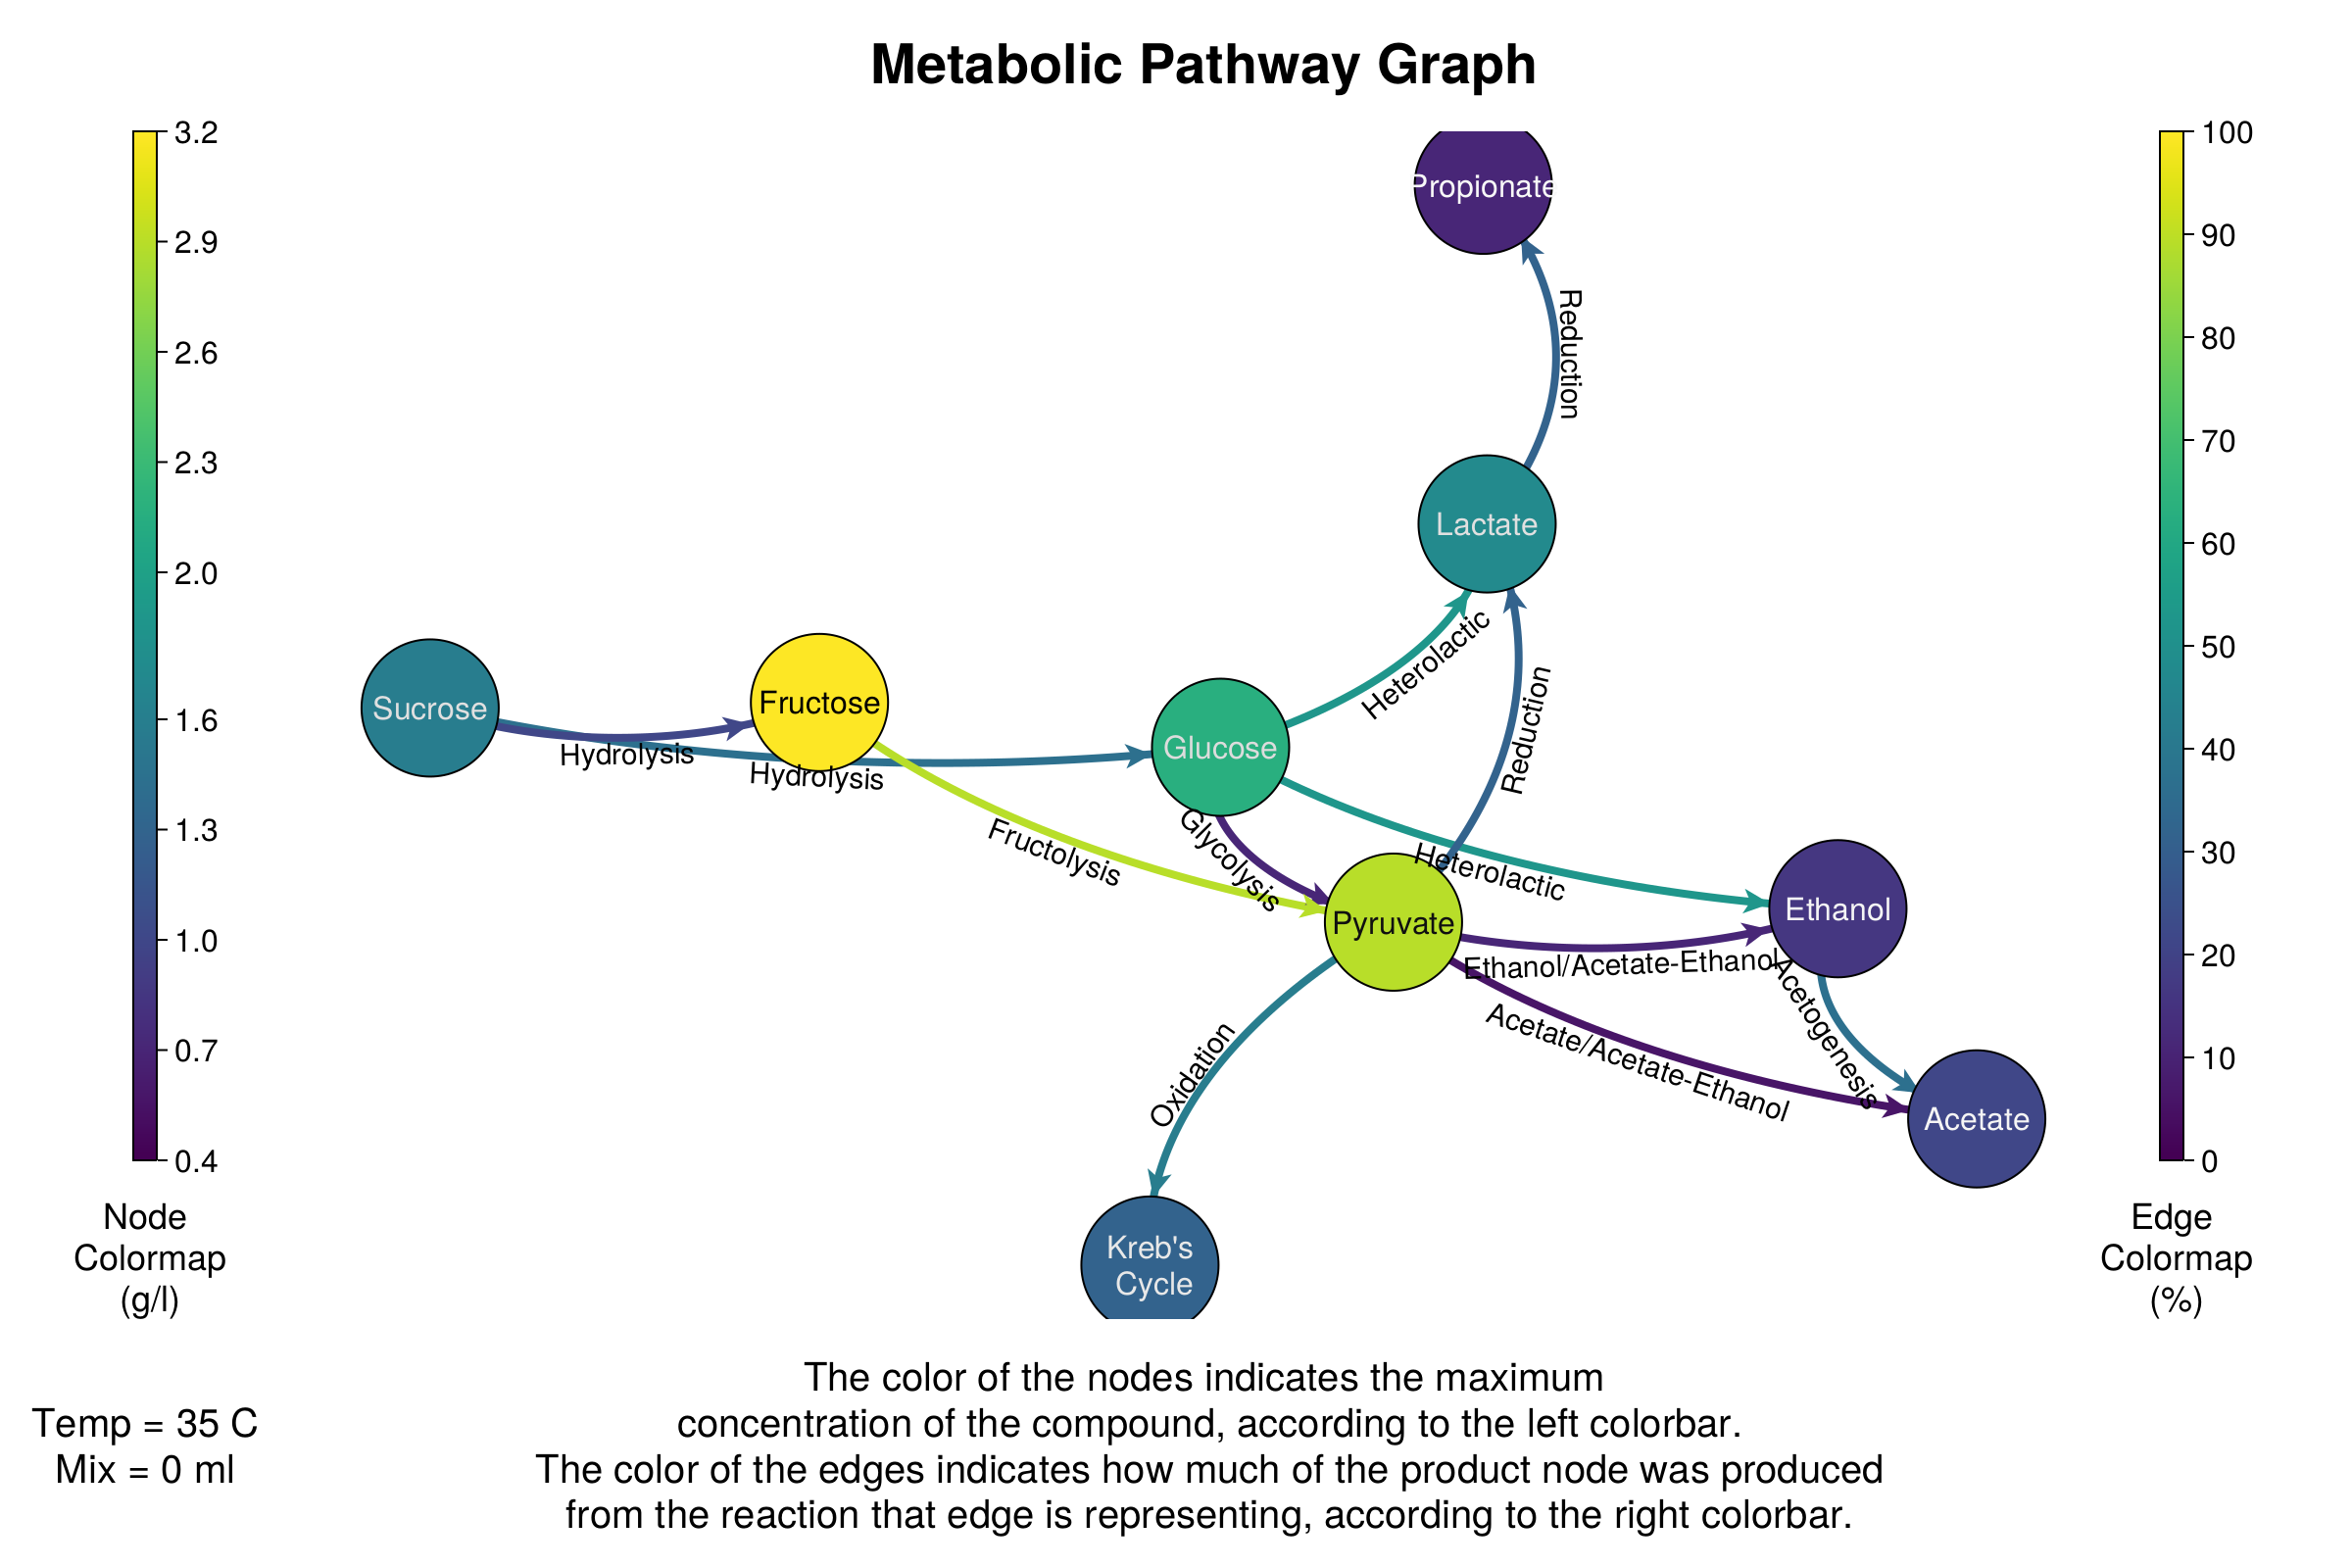
\includegraphics[width=.9\linewidth]{../plots/metabolic_results/35_0.png}
\end{center}

\section{Performing the result analysis on each dataset}
\label{sec:org28e635e}
This section has the goal of loading the jld2 file saved above and initializing all the necessary variables to do the result analysis (meaning generate the needed tables and plots). The majority of dependencies are in \texttt{metabolism\_results.jl}. DrWatson and JLD2 which are needed are not however.

\begin{minted}[breaklines=true,breakanywhere=true]{julia}

using DrWatson
@quickactivate "Masters_Thesis"
using JLD2
include(srcdir("metabolic_pathways", "metabolism_results.jl"))
\end{minted}

After dependencies, we can unpack the results.

\begin{minted}[breaklines=true,breakanywhere=true]{julia}

data_dir = wload(datadir("simulations", "metabolic_pathways.jld2"))

st35_0, df35_0, p35_0, v = data_dir["35_0"]
st35_1, df35_1, p35_1, v = data_dir["35_1"]
st35_2, df35_2, p35_2, v = data_dir["35_2"]
st35_4, df35_4, p35_4, v = data_dir["35_4"]
st35_8, df35_8, p35_8, v = data_dir["35_8"]

st40_0, df40_0, p40_0, v = data_dir["40_0"]
st40_1, df40_1, p40_1, v = data_dir["40_1"]
st40_2, df40_2, p40_2, v = data_dir["40_2"]
st40_4, df40_4, p40_4, v = data_dir["40_4"]
st40_8, df40_8, p40_8, v = data_dir["40_8"]
\end{minted}

\subsection{Generate the necessary tables}
\label{sec:orgd824732}
The above code for result analysis creates a lot of useful to have tables. I want to save 4 different table formats for each experiment. These are: The reaction flux table, the flux table containing the reactions as well as initial and final state, the "readable" flux table containing the labels of each column and row and the absolute flux table which is not normalized in (0, 1) but in the absolute concentration values measured. For simplicity, a helper function will be defined which runs all 4 and return the 4 tables and then only one function needs to be ran for each experiment.

\begin{minted}[breaklines=true,breakanywhere=true]{julia}

# Convenience code wrapping the process
function generate_flux_tables(st, df, p, v)
    rflux = reaction_fluxes(st, df, p, v)
    cflux = complete_fluxes(st, df, p, v)
    readflux = readable_flux_table(st, df, p, v)
    absflux = absolute_flux_table(st, df, p, v)

    rflux_t = Tables.table(rflux, header = [:SucHyd, :Glycolysis, :Heterolact, :PyrOx, :Acet, :Lact, :Eth, :Aceteth, :Prop, :Acetogenesis])
    cflux_t = Tables.table(cflux, header = [:Init, :SucHyd, :Glycolysis, :Heterolact, :PyrOx, :Acet, :Lact, :Eth, :Aceteth, :Prop, :Acetogenesis, :Final])
    absflux_t = Tables.table(absflux, header = [:Init, :SucHyd, :Glycolysis, :Heterolact, :PyrOx, :Acet, :Lact, :Eth, :Aceteth, :Prop, :Acetogenesis, :Final])

    # The readable flux table already has headers so that process
    # isn't necessary for it.
    return rflux_t, cflux_t, readflux, absflux_t
end

# Example generation of the tables
rflux35_0, cflux35_0, readflux35_0, absflux35_0 = generate_flux_tables(st35_0, df35_0, p35_0, v)
CSV.write(datadir("simulations", "flux_tables", "reaction_flux_table35_0.csv"), rflux35_0)
CSV.write(datadir("simulations", "flux_tables", "complete_flux_table35_0.csv"), cflux35_0)
CSV.write(datadir("simulations", "flux_tables", "readable_flux_table35_0.csv"), readflux35_0)
CSV.write(datadir("simulations", "flux_tables", "absolute_flux_table35_0.csv"), absflux35_0)

# Doing it for the rest of the datasets.
rflux35_1, cflux35_1, readflux35_1, absflux35_1 = generate_flux_tables(st35_1, df35_1, p35_1, v)
CSV.write(datadir("simulations", "flux_tables", "reaction_flux_table35_1.csv"), rflux35_1)
CSV.write(datadir("simulations", "flux_tables", "complete_flux_table35_1.csv"), cflux35_1)
CSV.write(datadir("simulations", "flux_tables", "readable_flux_table35_1.csv"), readflux35_1)
CSV.write(datadir("simulations", "flux_tables", "absolute_flux_table35_1.csv"), absflux35_1)

rflux35_2, cflux35_2, readflux35_2, absflux35_2 = generate_flux_tables(st35_2, df35_2, p35_2, v)
CSV.write(datadir("simulations", "flux_tables", "reaction_flux_table35_2.csv"), rflux35_2)
CSV.write(datadir("simulations", "flux_tables", "complete_flux_table35_2.csv"), cflux35_2)
CSV.write(datadir("simulations", "flux_tables", "readable_flux_table35_2.csv"), readflux35_2)
CSV.write(datadir("simulations", "flux_tables", "absolute_flux_table35_2.csv"), absflux35_2)

rflux35_4, cflux35_4, readflux35_4, absflux35_4 = generate_flux_tables(st35_4, df35_4, p35_4, v)
CSV.write(datadir("simulations", "flux_tables", "reaction_flux_table35_4.csv"), rflux35_4)
CSV.write(datadir("simulations", "flux_tables", "complete_flux_table35_4.csv"), cflux35_4)
CSV.write(datadir("simulations", "flux_tables", "readable_flux_table35_4.csv"), readflux35_4)
CSV.write(datadir("simulations", "flux_tables", "absolute_flux_table35_4.csv"), absflux35_4)

rflux35_8, cflux35_8, readflux35_8, absflux35_8 = generate_flux_tables(st35_8, df35_8, p35_8, v)
CSV.write(datadir("simulations", "flux_tables", "reaction_flux_table35_8.csv"), rflux35_8)
CSV.write(datadir("simulations", "flux_tables", "complete_flux_table35_8.csv"), cflux35_8)
CSV.write(datadir("simulations", "flux_tables", "readable_flux_table35_8.csv"), readflux35_8)
CSV.write(datadir("simulations", "flux_tables", "absolute_flux_table35_8.csv"), absflux35_8)

rflux40_0, cflux40_0, readflux40_0, absflux40_0 = generate_flux_tables(st40_0, df40_0, p40_0, v)
CSV.write(datadir("simulations", "flux_tables", "reaction_flux_table40_0.csv"), rflux40_0)
CSV.write(datadir("simulations", "flux_tables", "complete_flux_table40_0.csv"), cflux40_0)
CSV.write(datadir("simulations", "flux_tables", "readable_flux_table40_0.csv"), readflux40_0)
CSV.write(datadir("simulations", "flux_tables", "absolute_flux_table40_0.csv"), absflux40_0)

rflux40_1, cflux40_1, readflux40_1, absflux40_1 = generate_flux_tables(st40_1, df40_1, p40_1, v)
CSV.write(datadir("simulations", "flux_tables", "reaction_flux_table40_1.csv"), rflux40_1)
CSV.write(datadir("simulations", "flux_tables", "complete_flux_table40_1.csv"), cflux40_1)
CSV.write(datadir("simulations", "flux_tables", "readable_flux_table40_1.csv"), readflux40_1)
CSV.write(datadir("simulations", "flux_tables", "absolute_flux_table40_1.csv"), absflux40_1)

rflux40_2, cflux40_2, readflux40_2, absflux40_2 = generate_flux_tables(st40_2, df40_2, p40_2, v)
CSV.write(datadir("simulations", "flux_tables", "reaction_flux_table40_2.csv"), rflux40_2)
CSV.write(datadir("simulations", "flux_tables", "complete_flux_table40_2.csv"), cflux40_2)
CSV.write(datadir("simulations", "flux_tables", "readable_flux_table40_2.csv"), readflux40_2)
CSV.write(datadir("simulations", "flux_tables", "absolute_flux_table40_2.csv"), absflux40_2)

rflux40_4, cflux40_4, readflux40_4, absflux40_4 = generate_flux_tables(st40_4, df40_4, p40_4, v)
CSV.write(datadir("simulations", "flux_tables", "reaction_flux_table40_4.csv"), rflux40_4)
CSV.write(datadir("simulations", "flux_tables", "complete_flux_table40_4.csv"), cflux40_4)
CSV.write(datadir("simulations", "flux_tables", "readable_flux_table40_4.csv"), readflux40_4)
CSV.write(datadir("simulations", "flux_tables", "absolute_flux_table40_4.csv"), absflux40_4)

rflux40_8, cflux40_8, readflux40_8, absflux40_8 = generate_flux_tables(st40_8, df40_8, p40_8, v)
CSV.write(datadir("simulations", "flux_tables", "reaction_flux_table40_8.csv"), rflux40_8)
CSV.write(datadir("simulations", "flux_tables", "complete_flux_table40_8.csv"), cflux40_8)
CSV.write(datadir("simulations", "flux_tables", "readable_flux_table40_8.csv"), readflux40_8)
CSV.write(datadir("simulations", "flux_tables", "absolute_flux_table40_8.csv"), absflux40_8)
\end{minted}

\subsection{Create the graphs}
\label{sec:org91351b2}
The tables are useful to log the results and be able to revisit them at any point. But, they are not very easy to read. For this reason, the graph function were created because the graphs offer a powerful visualization technique of the table data. This code block generates these.

\begin{minted}[breaklines=true,breakanywhere=true]{julia}

f35_0 = generate_metabolic_graph(st35_0, df35_0, p35_0, v, T = "35 C", mix = "0 ml")
save(plotsdir("metabolic_results", "35_0.png"), f35_0)
f35_1 = generate_metabolic_graph(st35_1, df35_1, p35_1, v, T = "35 C", mix = "1 ml")
save(plotsdir("metabolic_results", "35_1.png"), f35_1)
f35_2 = generate_metabolic_graph(st35_2, df35_2, p35_2, v, T = "35 C", mix = "2 ml")
save(plotsdir("metabolic_results", "35_2.png"), f35_2)
f35_4 = generate_metabolic_graph(st35_4, df35_4, p35_4, v, T = "35 C", mix = "4 ml")
save(plotsdir("metabolic_results", "35_4.png"), f35_4)
f35_8 = generate_metabolic_graph(st35_8, df35_8, p35_8, v, T = "35 C", mix = "8 ml")
save(plotsdir("metabolic_results", "35_8.png"), f35_8)

f40_0 = generate_metabolic_graph(st40_0, df40_0, p40_0, v, T = "40 C", mix = "0 ml")
save(plotsdir("metabolic_results", "40_0.png"), f40_0)
f40_1 = generate_metabolic_graph(st40_1, df40_1, p40_1, v, T = "40 C", mix = "1 ml")
save(plotsdir("metabolic_results", "40_1.png"), f40_1)
f40_2 = generate_metabolic_graph(st40_2, df40_2, p40_2, v, T = "40 C", mix = "2 ml")
save(plotsdir("metabolic_results", "40_2.png"), f40_2)
f40_4 = generate_metabolic_graph(st40_4, df40_4, p40_4, v, T = "40 C", mix = "4 ml")
save(plotsdir("metabolic_results", "40_4.png"), f40_4)
f40_8 = generate_metabolic_graph(st40_8, df40_8, p40_8, v, T = "40 C", mix = "8 ml")
save(plotsdir("metabolic_results", "40_8.png"), f40_8)
\end{minted}

\section{Shifts in metabolic reactions from changing parameters}
\label{sec:org74c5c5e}
Having all this, we can conclude how the metabolic pathways change by varying a parameter.

35 C: Increasing the mix amount significantly inhibits acetogenic pathways (the main indication for this is ethanol to acetate which is seen to a large extent in 0 and 1 ml but vanishes after, but also pyruvate to acetate has a very small rate in anything but 1 ml) and to a lesser extent inhibits propionate production while promoting reducing reactions such as pyruvate to lactate (direct reduction) and ethanol (reduction of Acetyl-CoA, produced from pyruvate). Also, Fructose is consumed more effectively. This indicates that heterolactic fermentation is carried by the indigenous microorganisms of the FW (as its flux doesn't increase with mix amount) but this group of microorganisms isn't inhibited by the microorganisms we insert (seen by the small decreases in heterolactate flux). Lactate gets very high amounts in high mix amounts as both groups of microorganisms are capable of producing significant amount of lactate. The other reactions don't seem significantly affected. A detail that should be noted is that by using this flux-based analysis process which gets relative values and doesn't care as much about the differences between initial conditions, we see that the experiments at 2 ml and 8 ml yield almost identical results. The main difference is that there is a flux of 10\% of pyruvate going to acetate-ethanol type fermentation instead of pure ethanol (which is reflected by the fact that slightly more acetate is produced at 8 ml), but besides that, which is a minor change, the two have many similarities. This is very nicely indicated in the graph where none of the arrow color changes, but all the node color changes because the experiment at 2 ml had more sugars. This was also noticed when we did the yield plots which compared total products with total sugars and these two experiments gave the same results. Curiously, 4 ml yields worse results than both, but these show even further that increasing the max amount from 2 to 8 ml does nothing.

40 C: Heterolactic fermentation seems to be stagnant with mix amount again, strengthening the hypothesis that it is done by the indigenous microorganisms. Other pathways that produce ethanol however are inhibited here due to temperature and independently of mix amount. At 0 ml (indigenous) acetate production is mainly done together with ethanol (acetate-ethanol type fermentation) showing that pathway having the largest flux of anaerobic pyruvate consumption, so that pathway has some ethanol (although still not much). Once we add the other microorganisms, this pathway is strongly inhibited with ethanol being produced only from heterolactate and acetate being produced without co-products and at an increased flux. The reduction of pyruvate to lactate is also promoted, strengthening the hypothesis that the microorganisms we add are controling its rate. Acetogenesis also seems promoted but not significantly due to the small amounts of ethanol that are produced. Lactate's reduction to propionate seems almost identical in all mix amounts besides 0 ml, where it is lowered. If not for that, it would be trivial to assert that the indigenous microorganisms are the one producing propionate (which is supported by the fact that at 35 C the ones we add inhibit the reaction hence cannot be the ones catalyzing it), but this image assumes that adding the mix "activated" the reaction. One possible explanation however is that the experiment at 40 C and 0 ml mix had significantly less sugars than any other experiment which may mean that the lower flux is indicative of this behaviour.

One last thing that we notice is the relationship between ethanol and acetate. As mentioned above, in 35 C, acetate is inhibited while in 40 C ethanol is. In the assumed reaction system (which is based on literature), these two can be produced from pyruvate either separately or together. The acetate-ethanol type fermentation is notably a very important pathway in low pH and based on the results, the indigenous microorganisms, albeit capable of all 3 routes, cannot produce ethanol outside of this pathway in 40 C and cannot produce acetate outside of it at 35 C as their fluxes tend to 0 in these cases but are significant in the other temperature. This is no longer true if we add the mix. Acetate is produced at a decent rate at 1 ml mix at 35 C indicating that the pathway has been activated but not yet inhibited and small amounts of pure ethanol fermentation are seen at 1 and 2 ml mix at 40 C, although that inhibition appears to be stronger than that of acetate.

Some of these are visible if you look at the graph networks or the matrices generated above, but although the graph visualization is very nice and indicative, we don't want to have to show 9 identical looking graphs with only the colors changing, so we want some more fine-tuned graphs to be able to better summarize some results. These are shown below.

\subsection{Amount of glucose consumed in heterolactic fermentation}
\label{sec:org520486d}
The glucose being consumed in heterolactic fermentation is the majority of the total glucose and it's flux is very similar in all experiments, with its changes not being able to be attributed to the mix. Therefore, I believe it is done by the indigenous microorganisms. To indicate this better, we can plot how it changes in the various experiments. A bar plot is the ideal way to do this.

\begin{minted}[breaklines=true,breakanywhere=true]{julia}

gluc_fluxes = [p35_0[1], p35_1[1], p35_2[1], p35_4[1], p35_8[1], p40_0[1], p40_1[1], p40_2[1], p40_4[1], p40_8[1]]
x = 1:length(gluc_fluxes)
ticklabels = ["35 C\n 0 ml", "35 C\n 1 ml", "35 C\n 2 ml", "35 C\n 4 ml", "35 C\n 8 ml", "40 C\n 0 ml", "40 C\n 1 ml", "40 C\n 2 ml", "40 C\n 4 ml", "40 C\n 8 ml"]

het_plot = barplot(x, gluc_fluxes,
                   axis = (xticks = (x, ticklabels),
                           title = "% of Glucose Consumed in Heterolactic Fermentation",
                           limits = (nothing, (0.0, 0.9))))
save(plotsdir("metabolic_results", "heterolactate_flux.png"), het_plot)
\end{minted}

\begin{center}
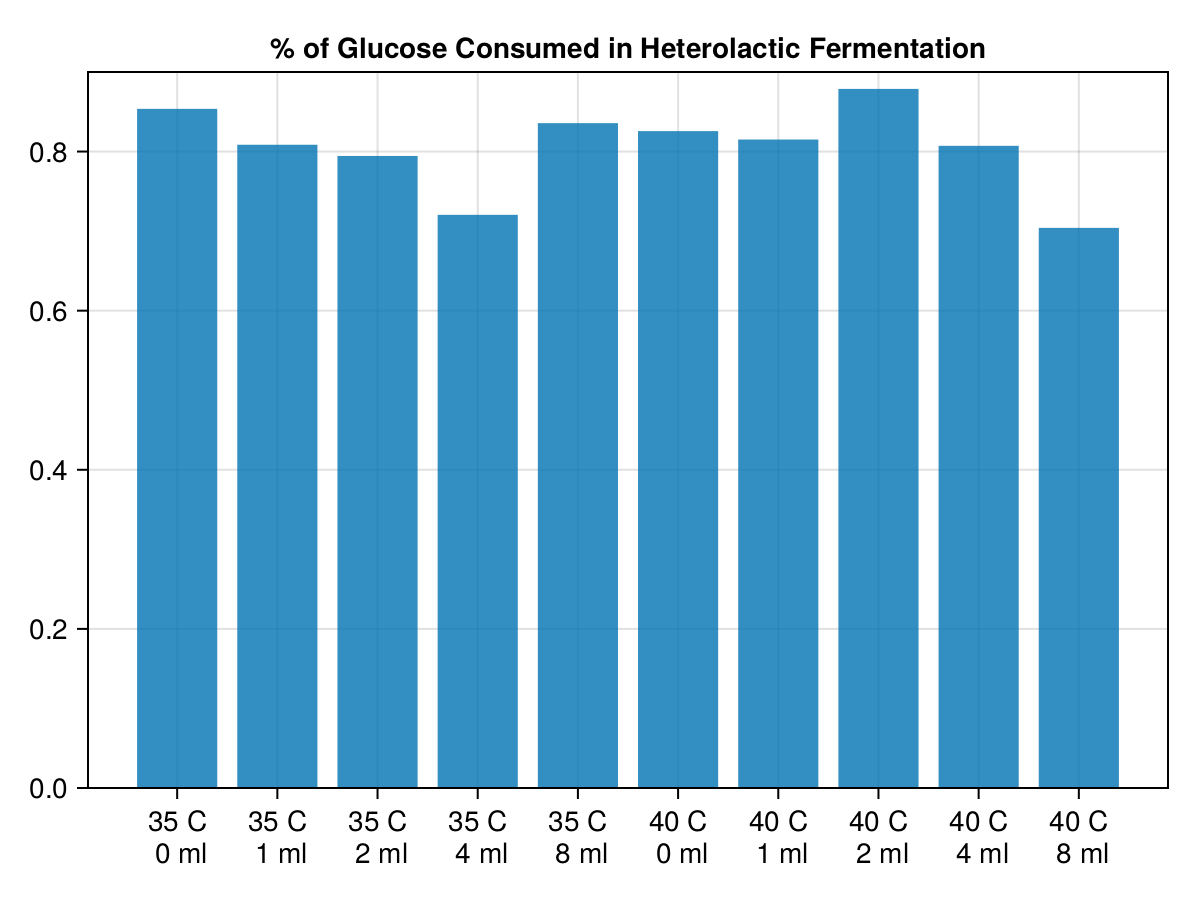
\includegraphics[width=.9\linewidth]{../plots/metabolic_results/heterolactate_flux.png}
\end{center}

In this plot it is evident that 8/10 are at 80\% or just above it (40 C/2 ml is slightly higher but not by too much) and then 2 diverge a bit by being lower, but even then, not by a very large extent. The standard deviation of the ten observations is only 0.05 which is definitely low enough to be called randomnes.

\subsection{Amount of lactate consumed for propionate production}
\label{sec:orgb1bb36b}
Propionate production shows signs of inhibition at 35 C (although to a lesser extent compared to acetate) and shows stagnation at 40 C after 1 ml. These are both plotted to indicate these.

\begin{minted}[breaklines=true,breakanywhere=true]{julia}

lact_cons35_0 = lactate_dist(st35_0, df35_0, p35_0, v)[3]
lact_cons35_1 = lactate_dist(st35_1, df35_1, p35_1, v)[3]
lact_cons35_2 = lactate_dist(st35_2, df35_2, p35_2, v)[3]
lact_cons35_4 = lactate_dist(st35_4, df35_4, p35_4, v)[3]
lact_cons35_8 = lactate_dist(st35_8, df35_8, p35_8, v)[3]

lact_cons40_0 = lactate_dist(st40_0, df40_0, p40_0, v)[3]
lact_cons40_1 = lactate_dist(st40_1, df40_1, p40_1, v)[3]
lact_cons40_2 = lactate_dist(st40_2, df40_2, p40_2, v)[3]
lact_cons40_4 = lactate_dist(st40_4, df40_4, p40_4, v)[3]
lact_cons40_8 = lactate_dist(st40_8, df40_8, p40_8, v)[3]

lact_fluxes = abs.([lact_cons35_0, lact_cons35_1, lact_cons35_2, lact_cons35_4, lact_cons35_8, lact_cons40_0, lact_cons40_1, lact_cons40_2, lact_cons40_4, lact_cons40_8])

prop_35_p = barplot(x[1:5], lact_fluxes[1:5],
                    axis = (xticks = (x[1:5], ticklabels[1:5]),
                            title = "% of Lactate Reduced to Propionate - 35 C"))

prop_40_p = barplot(x[6:10], lact_fluxes[6:10],
                    axis = (xticks = (x[6:10], ticklabels[6:10]),
                            title = "% of Lactate Reduced to Propionate - 40 C"))

save(plotsdir("metabolic_results", "propionate_flux_35.png"), prop_35_p)
save(plotsdir("metabolic_results", "propionate_flux_40.png"), prop_40_p)
\end{minted}

\begin{center}
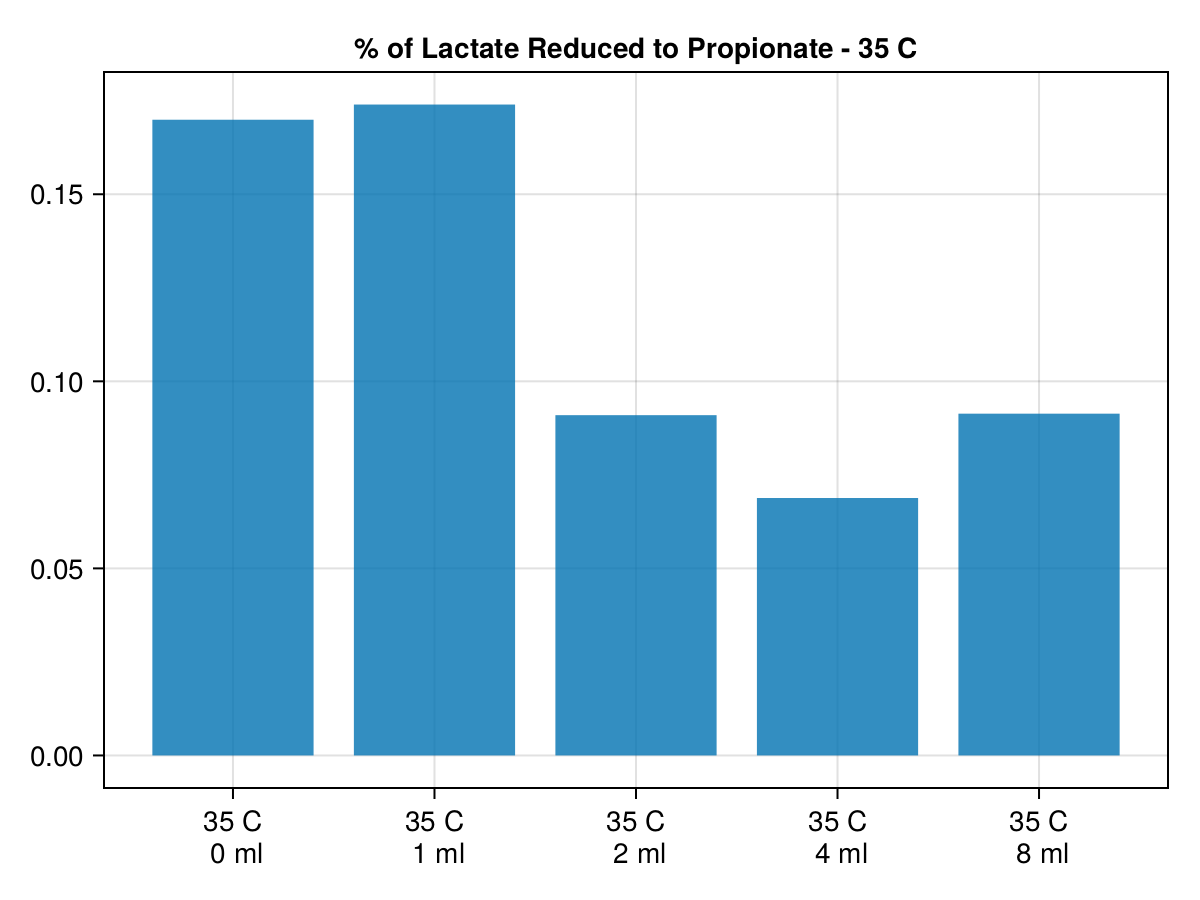
\includegraphics[width=.9\linewidth]{../plots/metabolic_results/propionate_flux_35.png}
\end{center}

\begin{center}
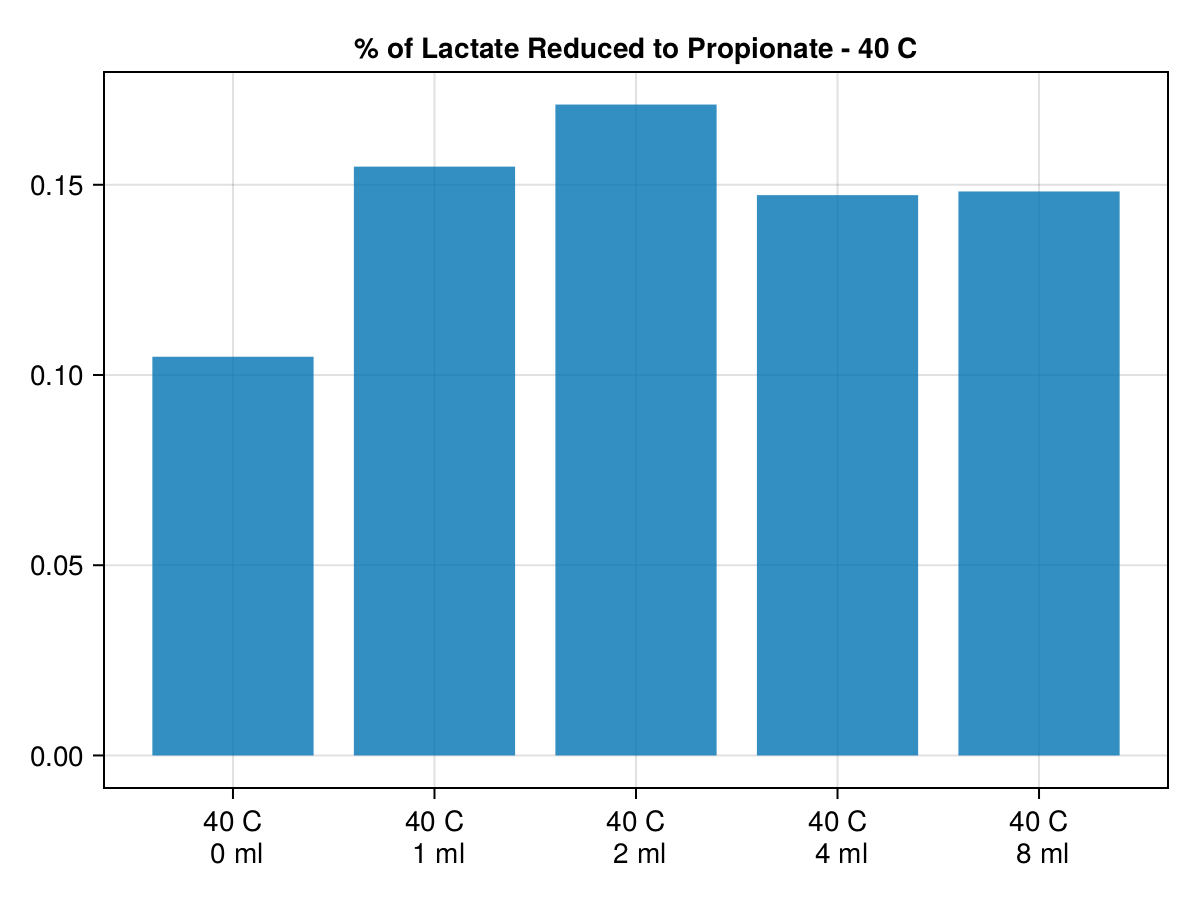
\includegraphics[width=.9\linewidth]{../plots/metabolic_results/propionate_flux_40.png}
\end{center}

\subsection{Pyruvate Flux Pie Plots}
\label{sec:org692dc50}
One of the things that we want to indicate is that acetate and ethanol fermentations act competitively between the two temperatures (meaning that one is strongly inhibited and the other strongly produced). But an interesting point (which is due to the indigenous microorganisms as it appears most evidently at 0 ml) is that if the inhibited one were to be produced, it would be produced in acetate/ethanol type fermentation, which is the 1:1 ratio fermentation producing both.  

\begin{minted}[breaklines=true,breakanywhere=true]{julia}

pyr35_0 = pyruvate_cons_dist(st35_0, df35_0, p35_0, v)
pyr35_1 = pyruvate_cons_dist(st35_1, df35_1, p35_1, v)
pyr35_2 = pyruvate_cons_dist(st35_2, df35_2, p35_2, v)
pyr35_4 = pyruvate_cons_dist(st35_4, df35_4, p35_4, v)
pyr35_8 = pyruvate_cons_dist(st35_8, df35_8, p35_8, v)

pyr40_0 = pyruvate_cons_dist(st40_0, df40_0, p40_0, v)
pyr40_1 = pyruvate_cons_dist(st40_1, df40_1, p40_1, v)
pyr40_2 = pyruvate_cons_dist(st40_2, df40_2, p40_2, v)
pyr40_4 = pyruvate_cons_dist(st40_4, df40_4, p40_4, v)
pyr40_8 = pyruvate_cons_dist(st40_8, df40_8, p40_8, v)

labels = ["Kreb's Cycle", "Acetate", "Lactate", "Ethanol", "Acetate/Ethanol\n type Fermentation"]
colors = Makie.wong_colors()[1:length(labels)]

pyr_ind_f = Figure(size=(600, 400))
Label(pyr_ind_f[1,1:3], "Pyruvate Flux Distribution for the \nindigenous microorganisms", fontsize = 20, font = :bold)
ax1, plt = pie(pyr_ind_f[2,1], pyr35_0, color = colors, axis = (aspect=DataAspect(), title = "35 C"))
ax2, plt = pie(pyr_ind_f[2,2], pyr40_0, color = colors, axis = (aspect=DataAspect(), title = "40 C"))
Legend(pyr_ind_f[2,3], [PolyElement(color=c) for c in colors], labels, framevisible=false)
hidedecorations!(ax1)
hidedecorations!(ax2)
hidespines!(ax1)
hidespines!(ax2)
save(plotsdir("metabolic_results", "pyr_flux_ind.png"), pyr_ind_f)

pyr_flux_f = Figure(size = (1350, 900))
Label(pyr_flux_f[1,1:3], "Pyruvate Flux Distribution", fontsize = 32, font = :bold)
Label(pyr_flux_f[2, 1:3], "Temperature = 35 C", fontsize = 25)

ax1, plt = pie(pyr_flux_f[3,1], pyr35_0, color = colors, axis = (aspect=DataAspect(), title = "0 ml", titlesize = 20))
ax2, plt = pie(pyr_flux_f[3,2], pyr35_1, color = colors, axis = (aspect=DataAspect(), title = "1 ml", titlesize = 20))
ax3, plt = pie(pyr_flux_f[3,3], pyr35_2, color = colors, axis = (aspect=DataAspect(), title = "2 ml", titlesize = 20))
ax4, plt = pie(pyr_flux_f[4,1], pyr35_4, color = colors, axis = (aspect=DataAspect(), title = "4 ml", titlesize = 20))
ax5, plt = pie(pyr_flux_f[4,2], pyr35_8, color = colors, axis = (aspect=DataAspect(), title = "8 ml", titlesize = 20))
hidedecorations!(ax1)
hidedecorations!(ax2)
hidedecorations!(ax3)
hidedecorations!(ax4)
hidedecorations!(ax5)
hidespines!(ax1)
hidespines!(ax2)
hidespines!(ax3)
hidespines!(ax4)
hidespines!(ax5)
Legend(pyr_flux_f[4:6,3], [PolyElement(color=c) for c in colors], labels, framevisible=false, labelsize = 22)

Label(pyr_flux_f[5, 1:3], "Temperature = 40 C", fontsize= 25)

ax6, plt = pie(pyr_flux_f[6,1], pyr40_0, color = colors, axis = (aspect=DataAspect(), title = "0 ml", titlesize = 20))
ax7, plt = pie(pyr_flux_f[6,2], pyr40_1, color = colors, axis = (aspect=DataAspect(), title = "1 ml", titlesize = 20))
ax8, plt = pie(pyr_flux_f[7,1], pyr40_2, color = colors, axis = (aspect=DataAspect(), title = "2 ml", titlesize = 20))
ax9, plt = pie(pyr_flux_f[7,2], pyr40_4, color = colors, axis = (aspect=DataAspect(), title = "4 ml", titlesize = 20))
ax10, plt = pie(pyr_flux_f[7,3], pyr40_8, color = colors, axis = (aspect=DataAspect(), title = "8 ml", titlesize = 20))
hidedecorations!(ax5)
hidedecorations!(ax6)
hidedecorations!(ax7)
hidedecorations!(ax8)
hidedecorations!(ax9)
hidedecorations!(ax10)
hidespines!(ax5)
hidespines!(ax6)
hidespines!(ax7)
hidespines!(ax8)
hidespines!(ax9)
hidespines!(ax10)

save(plotsdir("metabolic_results", "pyr_flux_tot.png"), pyr_flux_f)
\end{minted}

\begin{center}
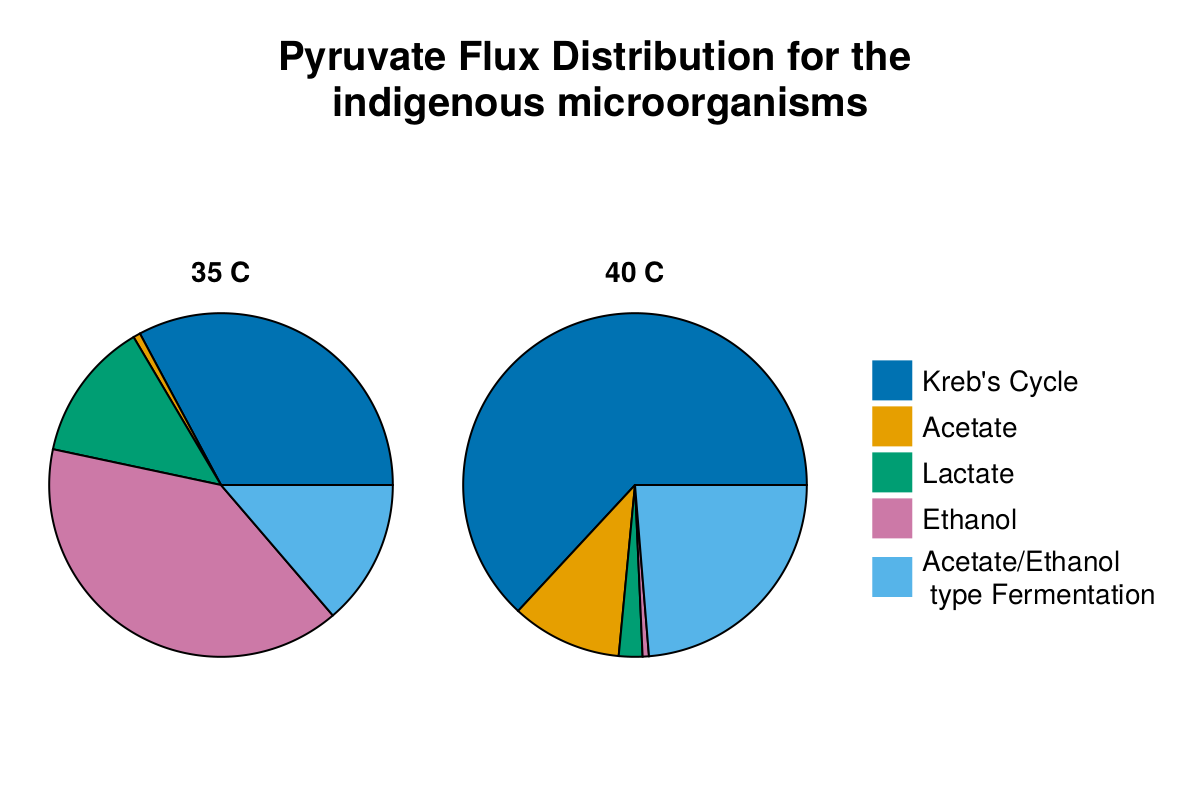
\includegraphics[width=.9\linewidth]{../plots/metabolic_results/pyr_flux_ind.png}
\end{center}

\begin{center}
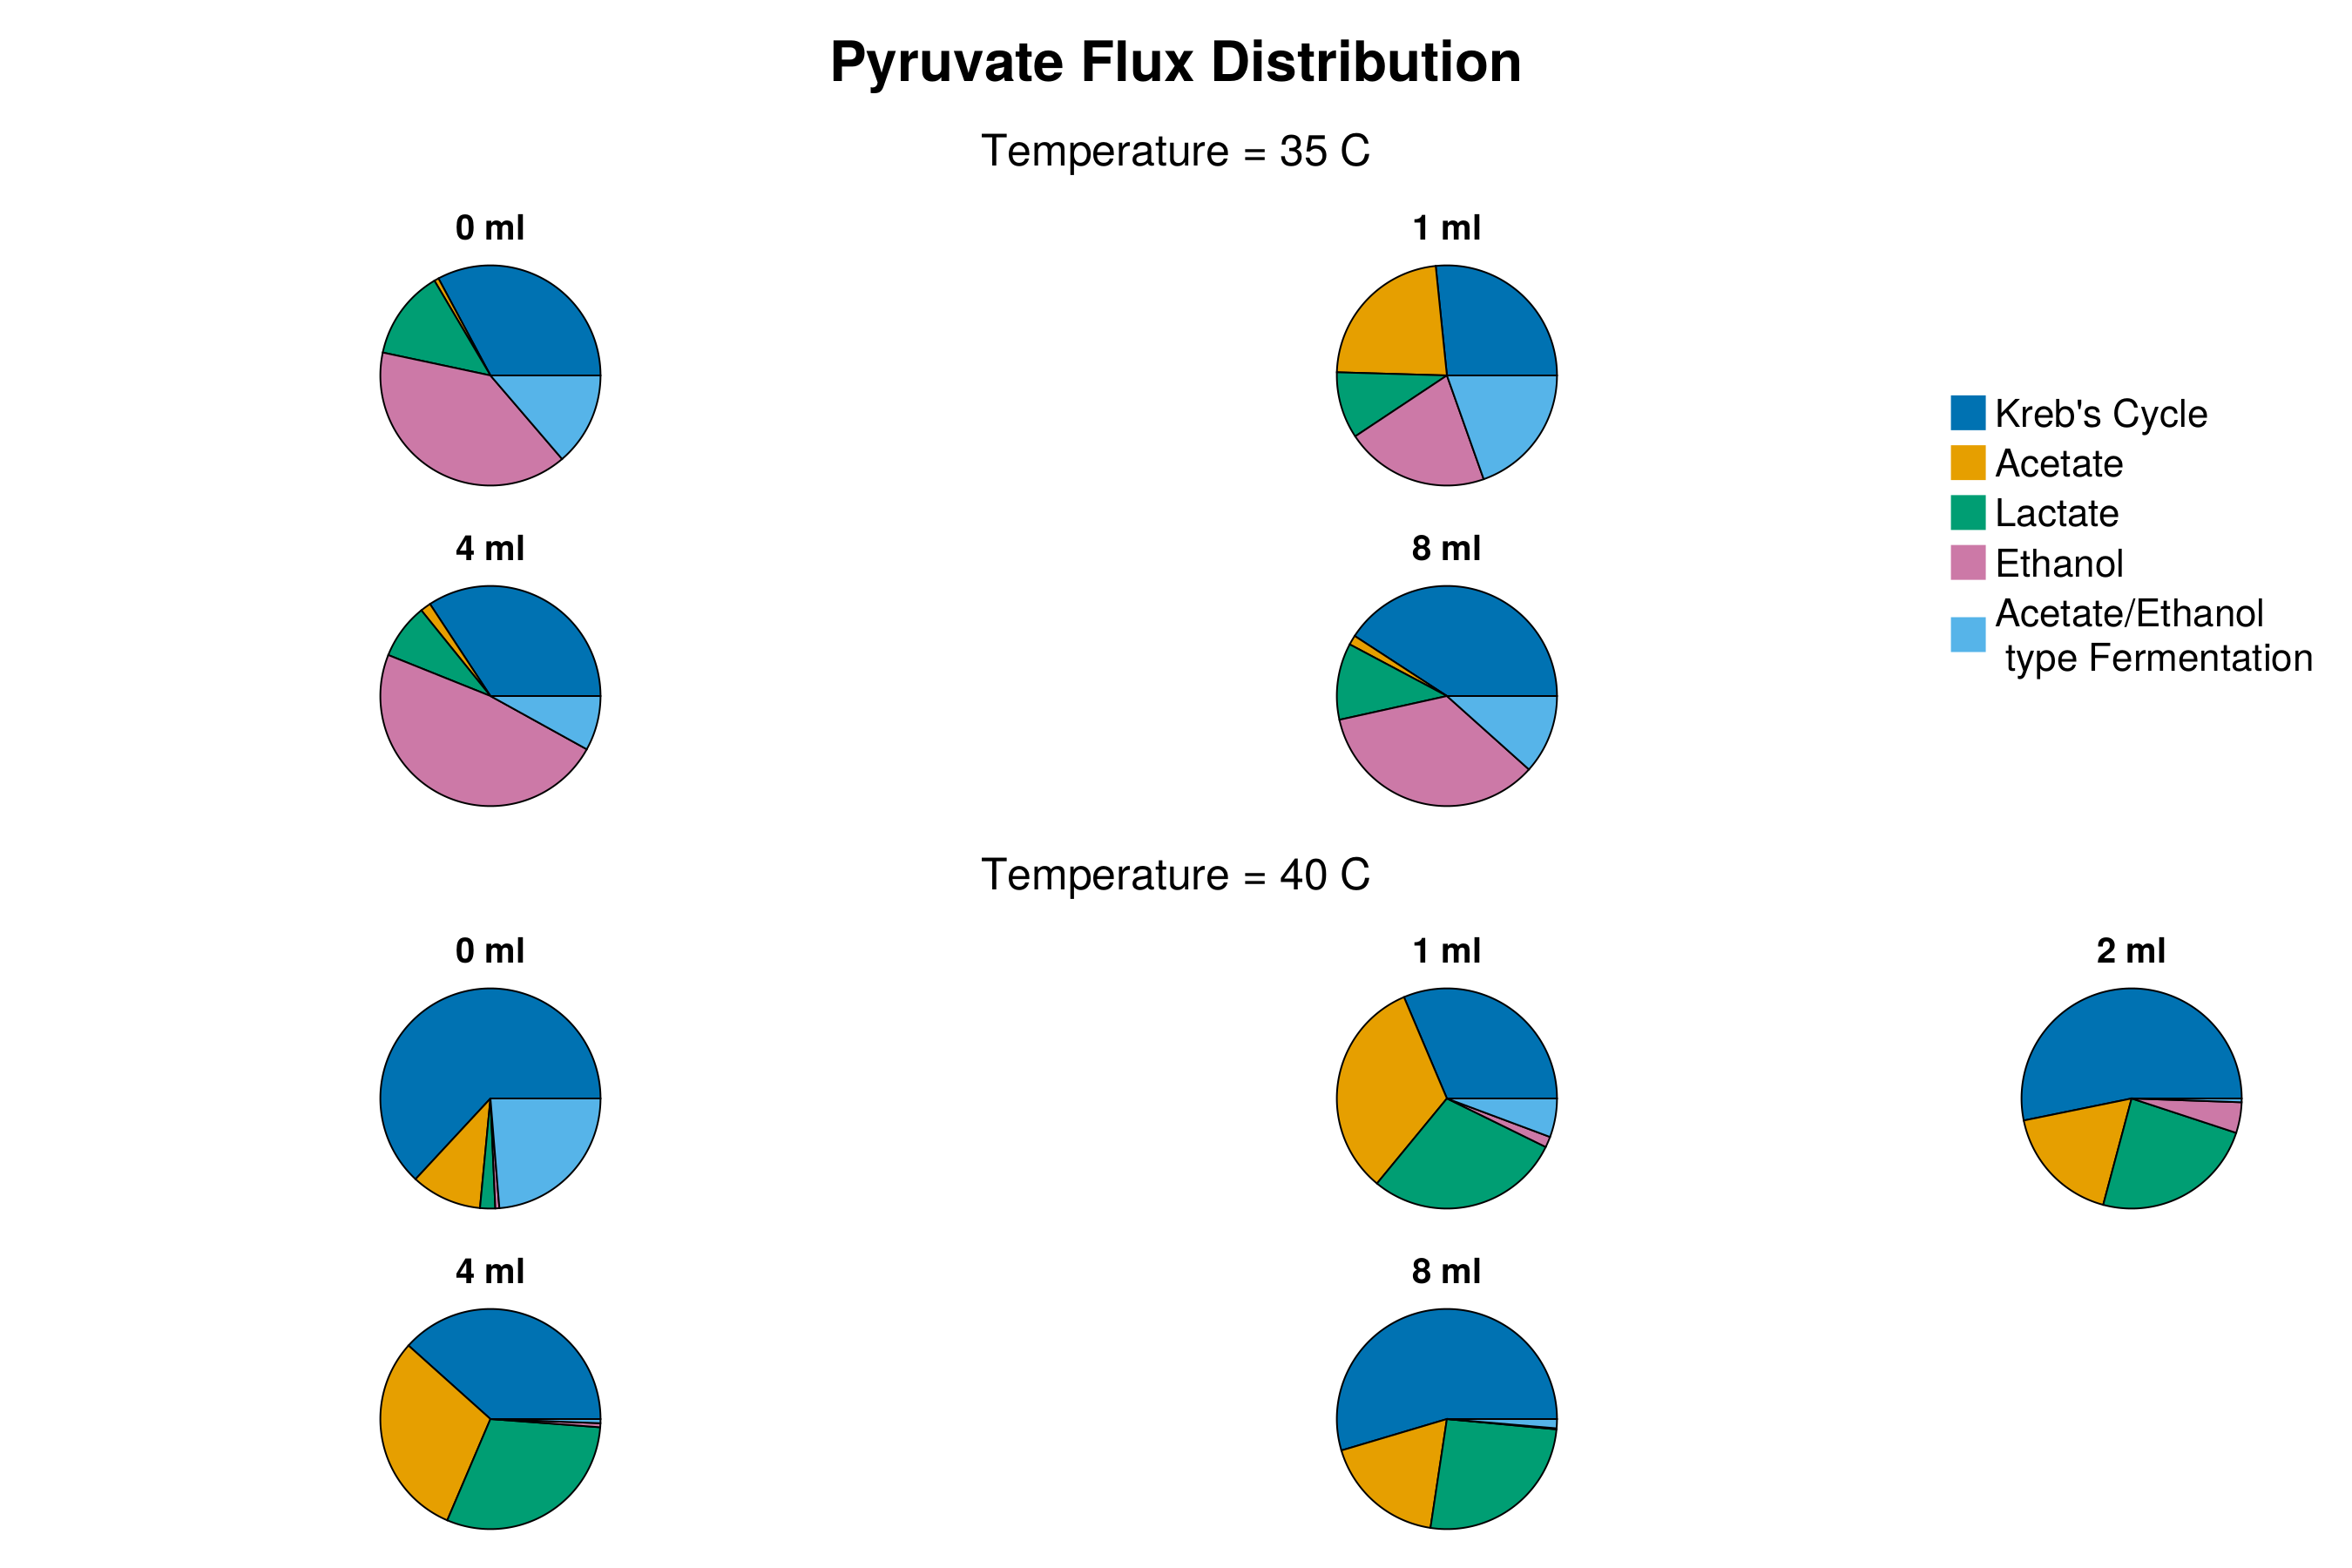
\includegraphics[width=.9\linewidth]{../plots/metabolic_results/pyr_flux_tot.png}
\end{center}

\section{General conclusions of the study}
\label{sec:orgf66268f}
After doing all the above work, we have basically concluded this project with some conclusions. Using information from literature about the possible pathways followed by our reaction system, we designed an infrastructure that with knowledge of to what extent each reaction was done, can predict the reactor effluent. The backwards problem of this formulation is that knowing the effluent of our reactor system we can predict to what extent each reaction was done. This backwards problem can easily be solved with the SciML tooling if formulated properly in Julia. With a robust local optimization method, we can bring the loss down to 1e-16/1e-20 in every case meaning a perfect prediction of the effluent. Having the results of this, we can design the metabolic pathway matrix which shows to which extent each compound is produced/consumed by each reaction, a very useful tool for this problem. From that matrix, we can draw our conclusions, as well as use visualization tools to support them.

The metabolic network graph created is a very nice image that contains a lot of information about our system all packed into one image. It is a very convenient representation of the results of this process without too many details. Other visualizations of the entire system are not necessary. However, more specific images are used to support some of the conclusions below.

The indigenous microorganisms can catalyze all 10 of the reactions we defined. However, the microorganisms contained in the mix only control some of them. Sucrose and Glucose are both consumed very fast in every case so it is very hard to assess if hydrolysis of sucrose and glycolysis are affected by the ones in the mix.
Heterolactic fermentation seems to only be done by the indigenous microorganisms as the ones we add seem to not affect its flux a significant amount. Fructolysis is definitely augmented by adding the mix as especially in 35 C, there remains Fructose in 72h, but is fully consumed if we add enough of the mix. Propionate production seems to be slightly affected by mix amount (especially in 35 C) but not significantly in any case so it's probably also done by the indigenous microorganisms (a plot indicating results for propionate in specific has been created) while the rest of the anaerobic metabolic reactions are definitely heavily affected by the prescence of the microorganisms in the mix.

One of the most important things we indicate (which however can be seen even without this analysis, but this gives us much more details on it) is the relationship between ethanol and acetate. It can very easily be noticed that in 35 C, acetate is inhibited while in 40 C ethanol is. In the assumed reaction system (which is based on literature), these two can be produced from pyruvate either separately or together. The acetate-ethanol type fermentation is notably a very important pathway in low pH and based on the results, the indigenous microorganisms, albeit capable of all 3 routes, cannot produce ethanol outside of this pathway in 40 C and cannot produce acetate outside of it at 35 C as their fluxes tend to 0 in these cases but are significant in the other temperature. This is no longer true if we add the mix. Acetate is produced at a decent rate at 1 ml mix at 35 C indicating that the pathway has been activated but not yet inhibited and small amounts of pure ethanol fermentation are seen at 1 and 2 ml mix at 40 C, although that inhibition appears to be stronger than that of acetate. However, it is interesting to see how the flux changes because one or the other isn't there.

In 35 C, most of the pyruvate flux can be attributed to ethanol production and then to lactate. However, when we go to 40 C, not all the flux of ethanol becomes acetate. It is separated between both acetate and lactate that are increased when ethanol isn't produced. And, the lactate at 40 C is higher than that at 35 C. This indicates that while the end products which are inhibited are ethanol and acetate depending on the temperature, it is not those 2 that are competing mainly, but ethanol and lactate. Assuming that flux can go into any of the three products, at 35 C, any flux that would go to acetate goes to ethanol due to its inhibition and that is because ethanol is more favoured than lactate as the reducing product of the process. Lactate flux also goes to ethanol in some conditions as seen for example in "35\textsubscript{4}". At 40 C, ethanol is inhibited so lactate takes over its flux. However, to have enough reducing potential, the acetate production pathway (which is oxidative) gets a large flux as well. In the previous case, ethanol didn't necessarily need to be paired with acetate because ethanol from pyruvate is a product of Acetyl-CoA, meaning it has already gotten the reductive potential acetate could provide. The acetate-ethanol paired pathway is feasible because the conversion of Acetyl-CoA to acetate is generally very energy feasible so even if we don't want acetate, it will be found as a co-product of ethanol. However, the conditions in the experiments from 2 ml and above at 35 C seem to inhibit acetate and therefore we see very large fluxes of ethanol produced without acetate.
\end{document}
